\documentclass[titlepage,a4paper]{article}

\usepackage{a4wide}
\usepackage[colorlinks=true,linkcolor=black,urlcolor=blue,bookmarksopen=true]{hyperref}
\usepackage{bookmark}
\usepackage{fancyhdr}
\usepackage[spanish]{babel}
\usepackage[utf8]{inputenc}
\usepackage[T1]{fontenc}
\usepackage{graphicx}
\usepackage{float}
\usepackage{tabularx}
\usepackage{tabto}
\usepackage{pgfgantt}
\usepackage{xcolor}
\usepackage{wrapfig}
\usepackage[utf8]{inputenc}
\usepackage{graphicx}
\usepackage{subcaption}



\pagestyle{fancy} % Encabezado y pie de página
\fancyhf{}
\fancyhead[L]{El Cuarteto Imperial - TP1}
\fancyhead[R]{75.06 Organización de Datos - FIUBA}
\renewcommand{\headrulewidth}{0.4pt}
\fancyfoot[C]{\thepage}
%\renewcommand{\footrulewidth}{0.4pt}
\renewcommand{\baselinestretch}{1,5}

\begin{document}
\begin{titlepage} % Carátula
    
	\hfill
\includegraphics[width=6cm]{logofiuba.jpg}
    \centering
    \vskip1cm
    \Huge \textbf{UBA - Facultad de Ingeniería}
    \vskip0.25cm
    \LARGE{Departamento de Computación}    
    \vskip0.25cm
    \LARGE{Organización de Datos (75.06)}
    \vskip1.2cm
    \vskip0.3cm
    \Huge \textbf{Trabajo Práctico 1} 
    \vskip0.5cm
    \LARGE{1er cuatrimestre - 2020}
    \vskip1.5cm
    \large
  	\begin{center}
    \begin{tabular}{||{7cm}||{2cm}||{6cm}||}
     \hline
     \multicolumn{3}{||c||}{GRUPO: \textbf{El Cuarteto Imperial}} \\ [0.5ex]
     \hline
     \hline
     \centering{\textbf{Alumno}} & \textbf{Padrón} & \textbf{Mail}\\ \hline
          LARREA BUENDÍA, Hugo Marcelo & 102140 & hlarrea@fi.uba.ar\\ \hline
          MARTINEZ SASTRE, Gonzalo Gabriel & 102321 & \normalsize gonzalomartinezsastre@gmail.com \\ \hline
          RIEDEL, Nicolás Agustín & 102130 & nriedel@fi.uba.ar\\ \hline
          ZBOGAR, Ezequiel & 102216 & ezbogar@fi.uba.ar\\ \hline
    \end{tabular}
    \end{center}
     
    \end{titlepage}
    
\tableofcontents
\newpage
\setlength{\parskip}{2mm}
\section{Resumen}\label{sec:resumen}
En el presente Trabajo Práctico se lleva a cabo un análisis exploratorio de datos en base a un set de datos compuesto por Tweets de diferentes partes del mundo.

El objeto de dicho análisis es organizar la información que aportan los datos de manera que sea plausible detectar patrones de comportamiento, tendencias, valores atípicos (también llamados outliers), resultados inesperados, saltos o discontinuidades, concentraciones de valores, formas de distribución, o cualquier otro tipo de característica destacable, de manera tal que permitan posteriormente elaborar conclusiones sobre los mismos.

A lo largo de este trabajo se [COMPLETAR CUANDO EL INFORME ESTE FINALIZADO]




\newpage

\section{Introducción}\label{sec:intro}
    El objetivo de este informe  es exponer los resultados del análisis exploratorio realizado en base al set de datos provisto por la cátedra. El mismo consiste en un conjunto de Tweets que se pueden hallar relacionados con desastres, ya sean de origen natural o provocado por el ser humano.
    
    La información provista por el set de datos para cada Tweet se describe a continuación: 
    
    \begin{itemize}
        \item \underline{Id}: Identificador único de cada Tweet.
        \item \underline{Texto}: Texto del Tweet.
        \item \underline{Locación}: El lugar desde el cual se mando el Tweet. 
        \item \underline{Keyword}: Una palabra particular del Tweet.
        \item \underline{Target}: Representa si el Tweet habla acerca de un desastre (1) o no (0)
    \end{itemize}
 
    En base a esto, se busca encontrar cualquier tipo de patrón o relación entre las distintas características de los Tweets (salvo el Id del Tweet debido a que éste es distinto para cada Tweet y no presenta información de interés).
    
    El lenguaje de programación utilizado fue Python. Adicionalmente, se utilizaron las siguientes herramientas: Git y Github como programas de control de versiones, Jupyter como entorno de desarrollo y las siguientes bibliotecas: Pandas, Numpy, Mathplotlib, Bokeh, PIL, Wordcloud, Math, Seaborn y Geopandas.
    
    Cabe destacar que a lo largo de todo este trabajo se tomó como convención llamar como verdaderos o veraces a aquellos Tweets que realmente tratan sobre un desastre, y como falsos o no veraces a aquellos que no lo hacen.
    
    
    \newpage
    \section{Análisis Léxico Gráfico de los Tweets}\label{sec:intro}
    Se comienza el análisis del conjunto de datos con un estudio del contenido de los Tweets. Para ello, como paso inicial se busca observar rasgos superficiales de los mismos, tales como la extensión de su texto tanto en palabras como en caracteres.
    
    [CAMBIAR TITULO DEL GRÁFICO O NO]
    
    \begin{figure}[H]
    \centering
    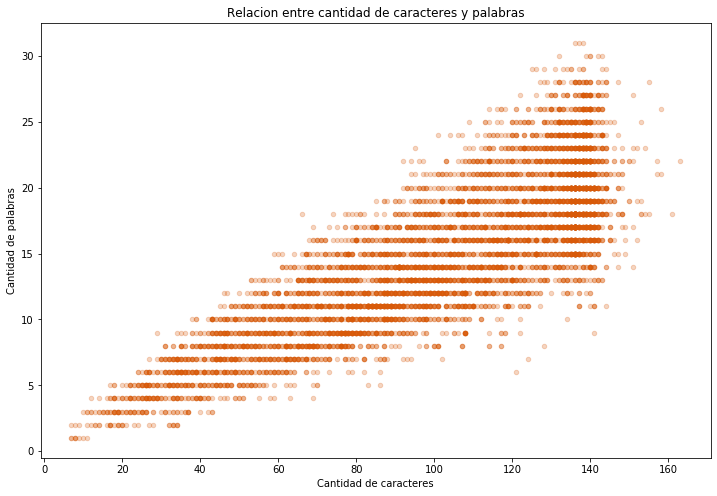
\includegraphics[width=1\textwidth]{graficos/Analisis Lexico Grafico/relacion_entre_cantidad_caracteres_palabras.png}
    \caption{}  
    \end{figure}
    
    En esta visualización cada punto representa un Tweet de los 7613 que conforman el set de datos. Como se puede observar, no se muestra ningún resultado inesperado puesto que es entendible que los Tweets con mayor cantidad de palabras tiendan a estar compuestos por un mayor número de caracteres.
    
    A continuación, se procede a realizar un estudio en profundidad del contenido de los mismos, primero buscando las palabras más repetidas (sin distinguir entre mayúsculas y minúsculas) con el objetivo de detectar temáticas predominantes. El resultado obtenido fue el siguiente:
    
    \begin{figure}[H]
    \centering
    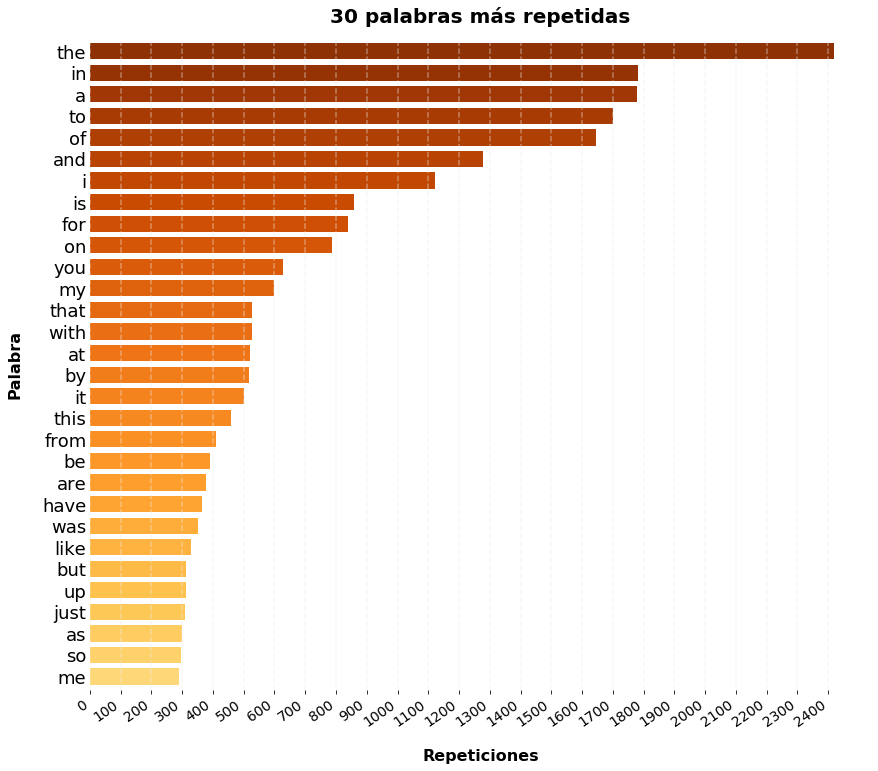
\includegraphics[width=1\textwidth]{graficos/Analisis Lexico Grafico/top30MasUsadas.png}
    \caption{}  
    \end{figure}
    
    Este resultado es el esperado, debido a que en el idioma ingles (el predominante en el set de datos) las palabras mas usadas son preposiciones.
    
    Ahora, se vuelve a generar el mismo gráfico pero filtrando preposiciones mediante un algoritmo. Esto me genera :
    
    \begin{figure}[H]
    \centering
    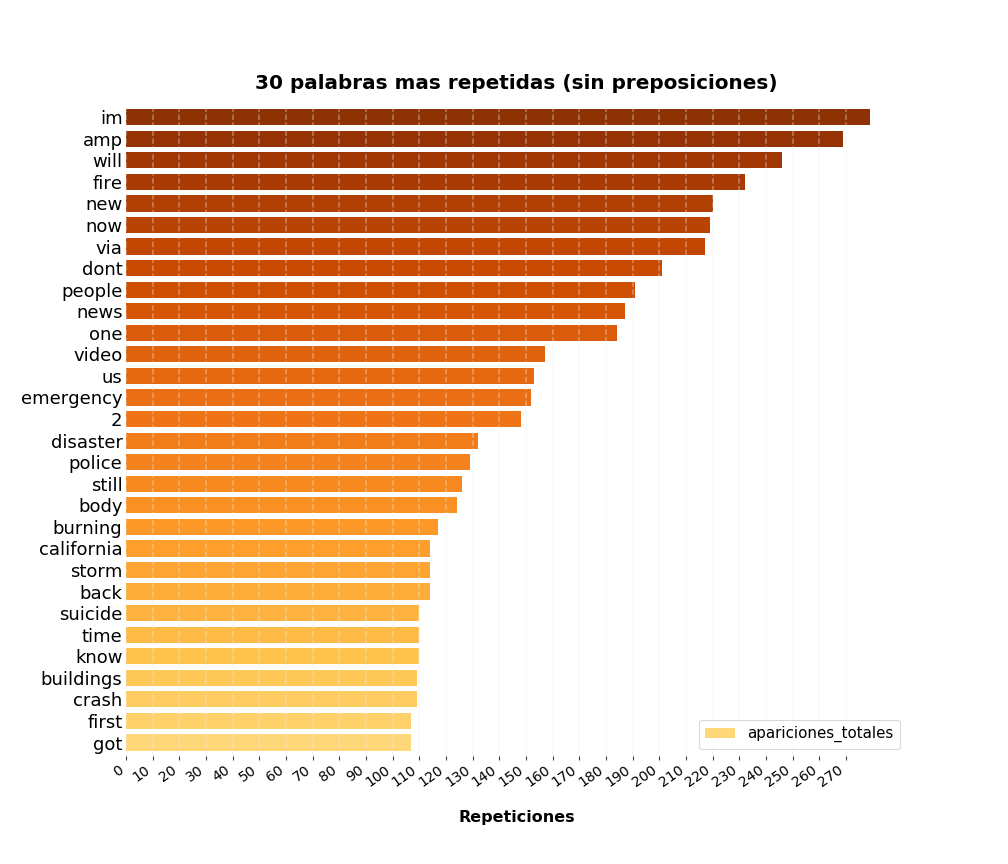
\includegraphics[width=1\textwidth]{graficos/Analisis Lexico Grafico/30masRepetidasFiltrado.png}
    \caption{}  
    \end{figure}
    
    Esto también es esperado, la mayoría de las palabras están relacionadas a desastres o a la comunicación de los mismo, que es el contenido del set de datos.
    
    Sin embargo, contando con un número de palabras tan alto (cerca de 30 mil palabras diferentes), el acotado grupo de elementos mostrado en la visualización anterior puede no ser una representación adecuada para el reconocimiento de patrones lingüísticos. Por ende, se realiza el wordcloud que se muestra a continuación :
    
     \begin{figure}[H]
    \centering
    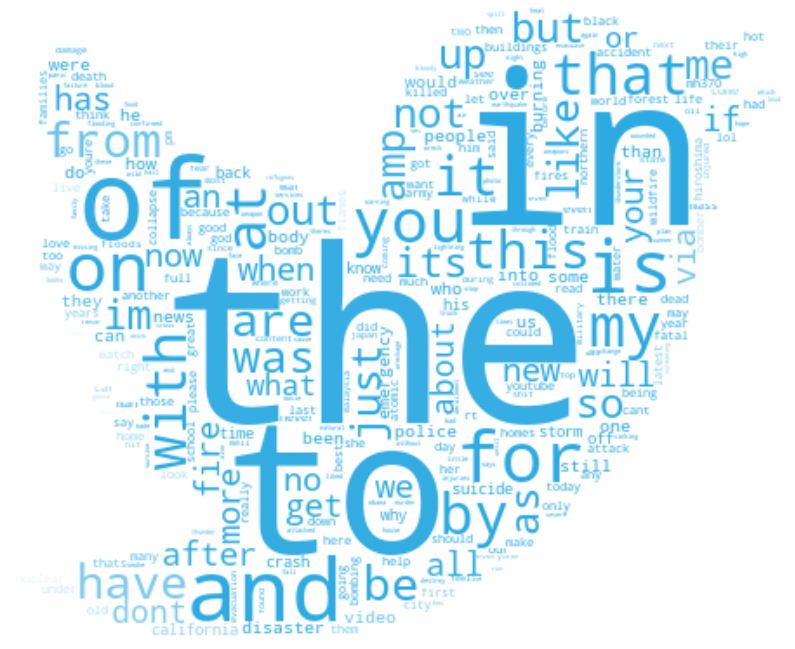
\includegraphics[width=1\textwidth]{graficos/Analisis Lexico Grafico/PalabrasMasUsadasSinFiltro.png}
    \caption{Tamaño proporcional al numero de repeticiones}
    \end{figure}
    
    Después, realizamos el mismo gráfico pero habiendo filtrado las preposiciones :
    
    \begin{figure}[H]
    \centering
    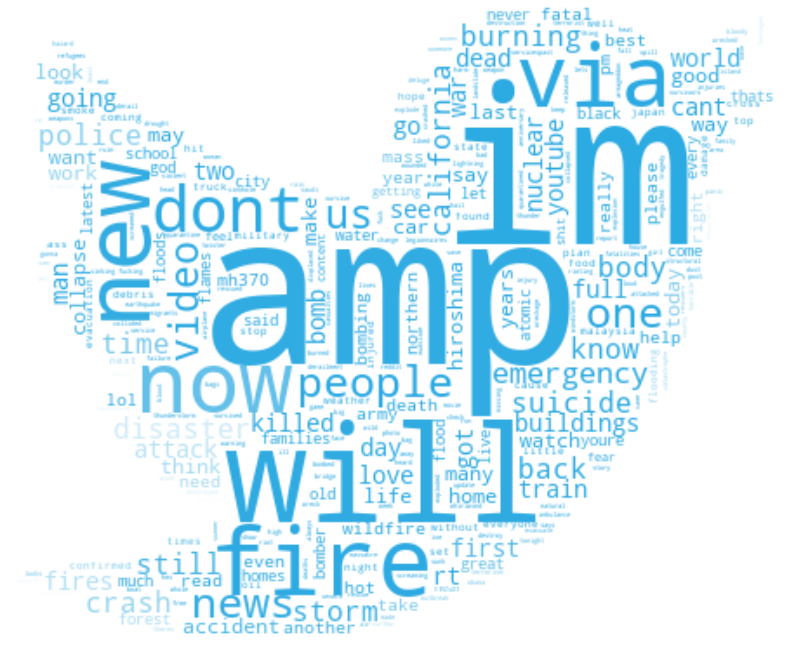
\includegraphics[width=1\textwidth]{graficos/Analisis Lexico Grafico/PalabrasMasUsadasConFiltro.png}
    \caption{Tamaño proporcional al numero de repeticiones}
    \end{figure}
    
    Habiendo estudiado el contenido de los Tweets en términos de palabras y prolongación, resultó de gran interés observar la relación de estos campos con los Tweets que tratan sobre un desastre real y aquellos que no lo hacen (aspecto que se considera como veracidad o target).
    
    No obstante, en primer lugar, es primordial estudiar la veracidad global de los Tweets como se muestra en la siguiente visualización.
    
    \begin{figure}[H]
    \centering
    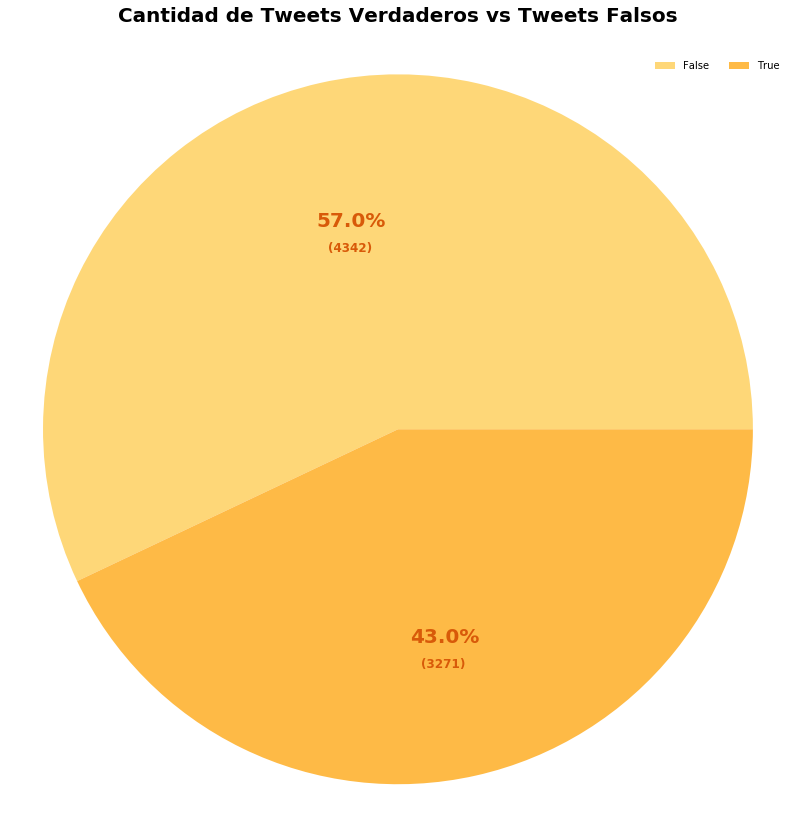
\includegraphics[width=1\textwidth]{graficos/Analisis Lexico Grafico/cantidad_de_tweets_verdadeos_vs_falsos.png}
    \end{figure}
    
    En un primer acercamiento a la veracidad de los Tweets, se puede apreciar que la mayoría de éstos no hacen referencia a ningún tipo de desastre. A pesar de ello, es destacable que dentro del set de datos la cantidad de Tweets para ambos casos es bastante pareja pues presentan una diferencia de 1071 Tweets en términos absolutos y de 14\% en términos relativos.
    
    Con esto observado, se puede proceder a buscar relaciones entre la veracidad de los Tweets y los distintos aspectos del texto de los mismos.
    
    El primer análisis que se efectúa tiene como objetivo el poder identificar si existe una conexión entre la frecuencia con la que se repiten las palabras y la veracidad de los Tweets que las contienen.
    

    [Cambiar titulo del gráfico]
    
    \begin{figure}[H]
    \centering
    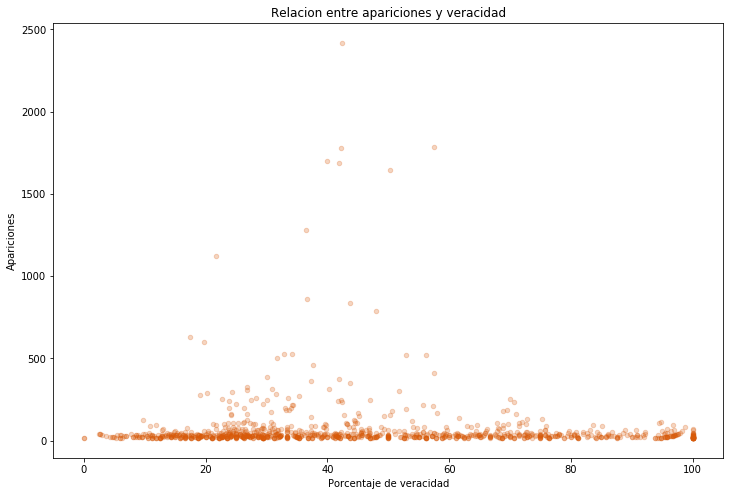
\includegraphics[width=1\textwidth]{graficos/Analisis Lexico Grafico/relacion_entre_apariciones_y_veracidad_2.png}
    \caption{} 
    \end{figure}
    
    Como se puede observar en este gráfico de dispersión, hay muy pocas palabras que aparecen mas de 500 veces, y dichas palabras tienen una veracidad cerca de la media. Por lo tanto no tienen impacto en un análisis relacionado a desastres. Es importante aclarar que si una apalabra aparece mas de una vez en el mismo tweet, esto de todas formas es considerado como una sola aparición de dicha palabra.
    
    Filtramos por palabras que aparecen menos de 500 veces. 
        
    \begin{figure}[H]
    \centering
    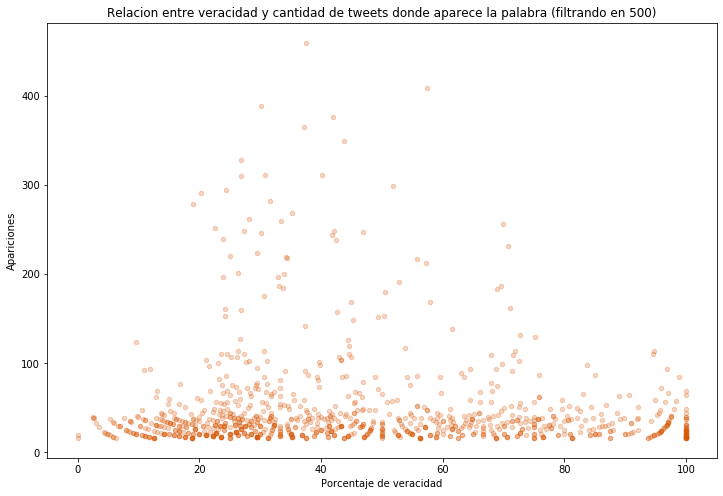
\includegraphics[width=1\textwidth]{graficos/Analisis Lexico Grafico/relacion_entre_apariciones_y_veracidad_filt_500.png}
    \caption{}   
    \end{figure}
    
    Al igual que en el gráfico anterior, se pude seguir observando que pasando las 100 apariciones no se encuentran palabras que tengan una veracidad interesante.
    
    \begin{figure}[H]
    \centering
    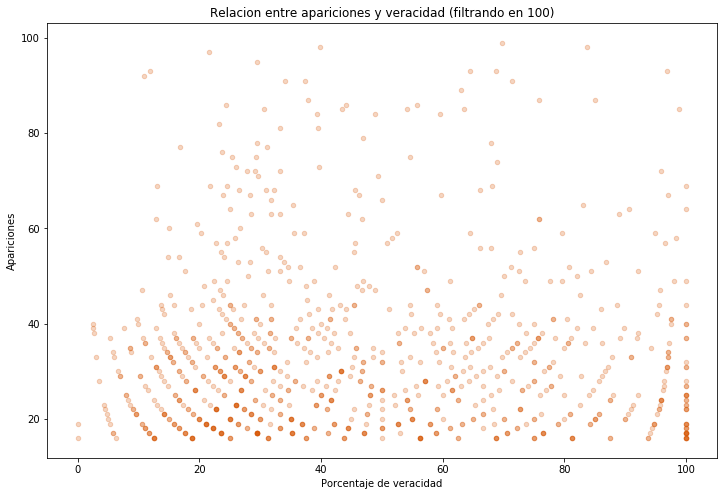
\includegraphics[width=1\textwidth]{graficos/Analisis Lexico Grafico/relacion_entre_aparicion_y_veracidad_filt_100.png}
    \caption{}
    \end{figure}
    
    En este gráfico se pueden observar cosas muy interesantes. Lo primero es que las palabras con mas apariciones tienden a rondar la media de veracidad, por lo tanto tienen poco impacto en un análisis del target.
    Por otro lado se pueden observar con claridad unas curiosas curvas, esto es debido a que el porcentaje de veracidad asociado a una palabra se calcula como el cociente entre apariciones veraces y apariciones totales. Siendo el eje vertical del gráfico las apariciones totales y el eje horizontal el porcentaje de veracidad, esto genera una relación de y = 1/x entre ambas variables.
    
    Un análisis que puede resultar de mayor interés consiste en encontrar cuales son las palabras con mayor veracidad asociada, es decir las que suelen aparecer mucho mas en tweets que hablan sobre desastres que en tweets que no lo hacen. En la visualización a continuación se procede a mostrar las palabras que solo aparecen en tweets veraces, cabe destacar que se decidido no mostrar las palabras que tienen menos de un 0.2\% de ocurrencias (aparecer en 12 tweets como mínimo para este caso). La razón de este filtro es evitar que aparezcan palabras que puedan llegar a tener alto \% de veracidad solo por aparecer pocas veces.
    
 
    
    \begin{figure}[H]
    \centering
    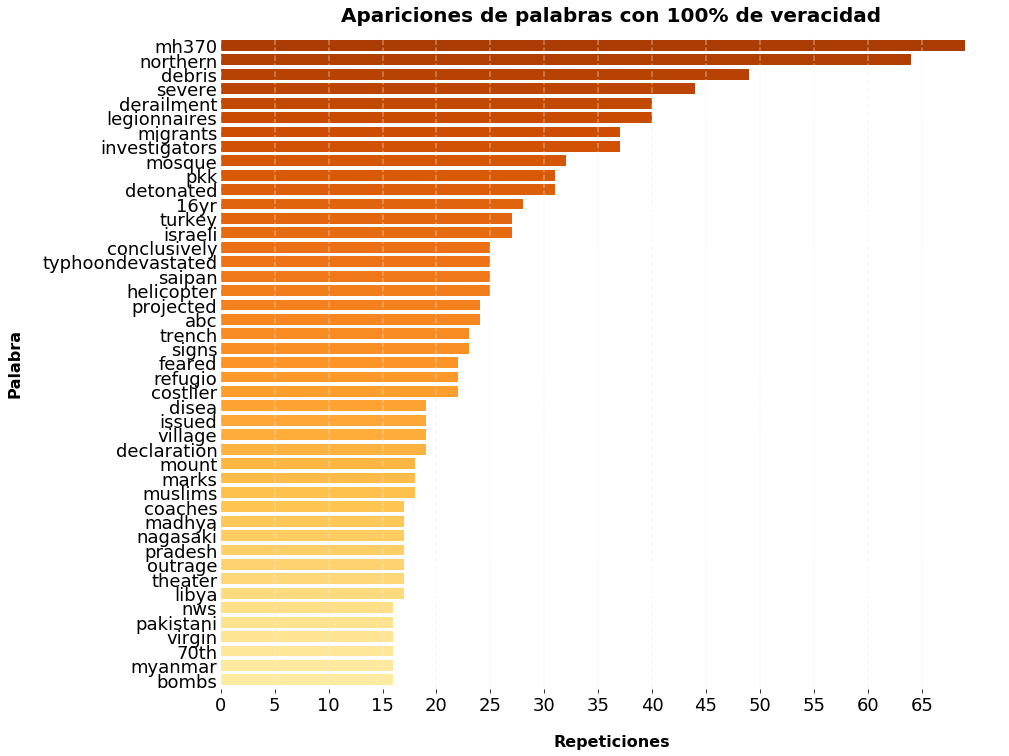
\includegraphics[width=1\textwidth]{graficos/Analisis Lexico Grafico/aparaciones_de_palabras_con_100_de_veracidad.png}
    \caption{Palabras 100\% veraces (Siempre que aparecen el tweet es verdadero)}
    \end{figure}
    
    Se aprecia que la palabra con mayor repeticiones que aparece solo en Tweets verídicos es ''mh370'', esta hace referencia al vuelo 370 de la aerolínea Malaysia Airlines que desapareció por causas desconocidas 8 de Marzo de 2014. Esto es razonable debido a ser un accidente que tuvo una gran difusión mediática. El resto de palabras están también altamente relacionadas con desastres, lo cual era de esperar. 
    
    Para una mayor exhibición, en el siguiente gráfico se pueden observar aquellas palabras cuyas apariciones en Tweets rondan entre el 90 y 100\% de veracidad. El tamaño de cada una esta relacionado con la cantidad de repeticiones (teniendo en cuenta convención mencionada previamente) y el color, como indica la barra inferior del gráfico, esta relacionada con el porcentaje de veracidad del total de Tweets que las contenían.
    \begin{figure}[H]
    \centering
    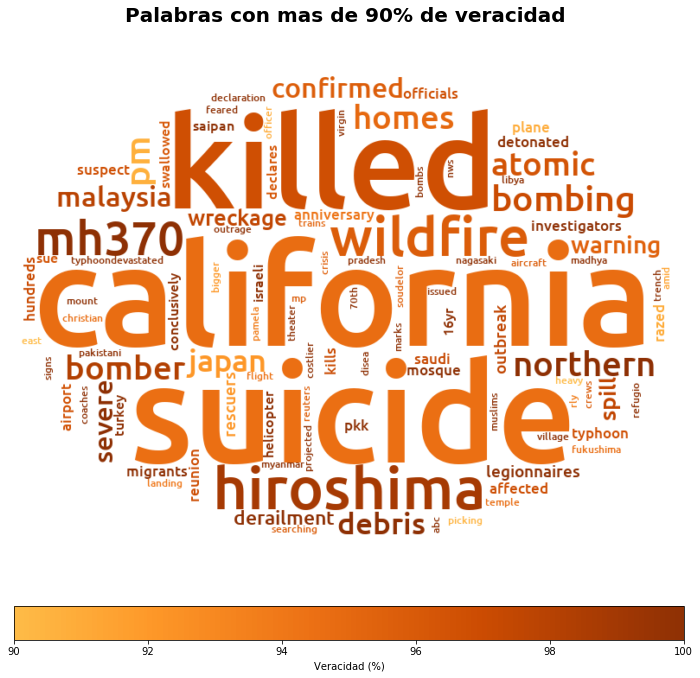
\includegraphics[width=1\textwidth]{graficos/Analisis Lexico Grafico/palabras_con_mas_de_90_de_veracidad.png}
    \caption{} 
    \end{figure}
    
    Como contraposición a las palabras con mayor índice de veracidad se pueden estudiar aquellas que sean completamente lo opuesto, es decir, las palabras cuyo porcentaje de veracidad en relación al total de Tweets en los que aparecen es muy bajo. 
    
    
    \begin{figure}[H]
    \centering
    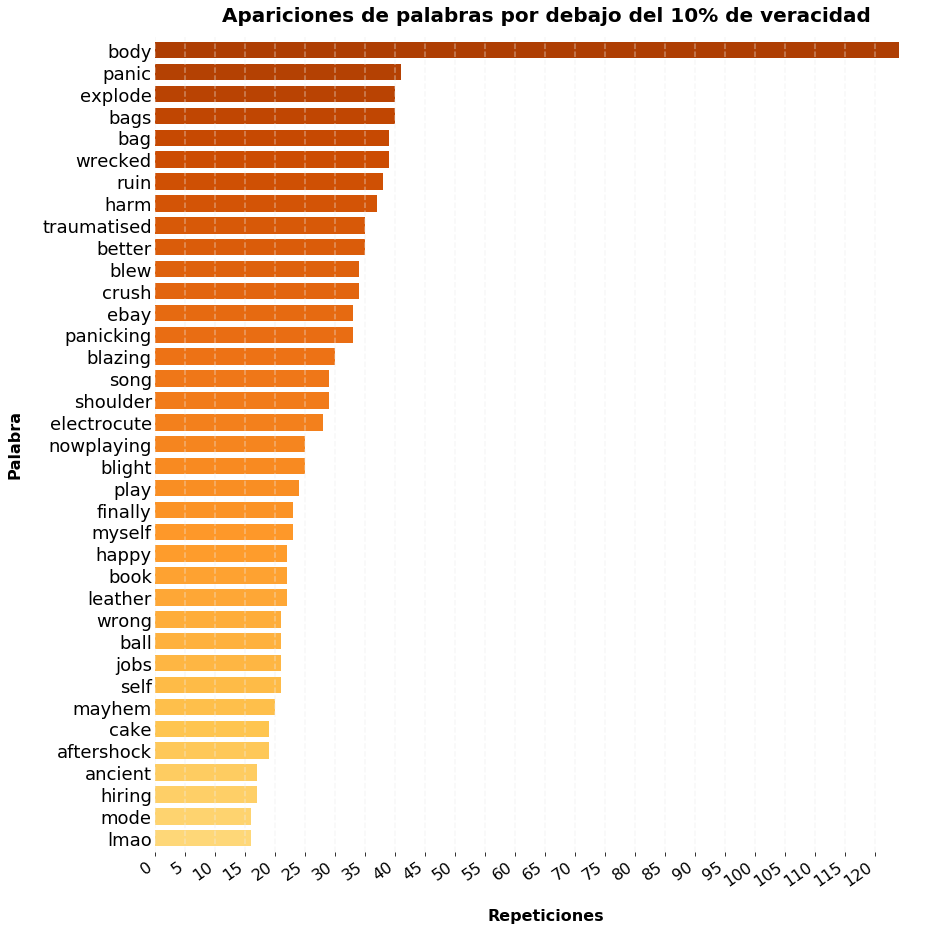
\includegraphics[width=1\textwidth]{graficos/Analisis Lexico Grafico/apariciones_de_palabras_por_debajo_de_10_de_veracidad.png}
    \caption{} 
    \end{figure}
    Como se puede apreciar y en contraste con lo dicho  para palabras con alto porcentaje de veracidad, las palabras con menos de 10\% de veracidad están en su mayoría poco relacionadas a un lenguaje esperable al hablar de una tragedia como por ejemplo ''cake'', ''ebay'' o ''song''. Otras palabras mayormente relacionadas con tragedias que se encuentran en este gráfico podría deberse al uso coloquial que se les da y el cual no esta relacionado necesariamente con un desastre (por ejemplo, la palabra ''crush'' en un Tweet podría hacer referencia a un siniestro automovilístico o bien a un interés romántico de la persona que lo redacto).
    

    En un intento de hilar mas fino, podemos quedarnos solo con las palabras que tienen menos de un 5\% de veracidad asociada. Esto quiere decir que solamente en un  5\% de los casos donde un tweet contiene esta palabra el mismo es veraz. 
    
    \begin{figure}[H]
    \centering
    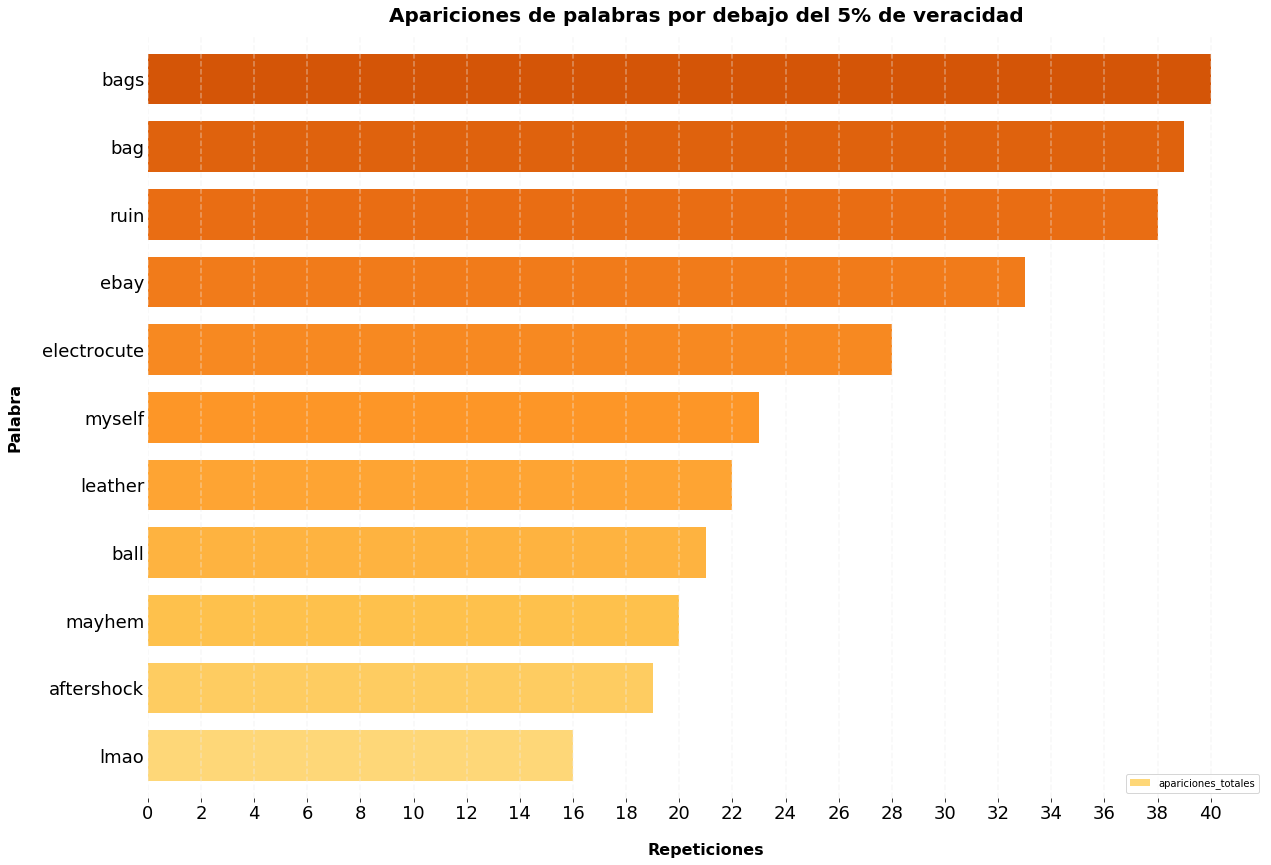
\includegraphics[width=1\textwidth]{graficos/Analisis Lexico Grafico/apariciones_de_palabras_por_debajo_de_5_de_veracidad.png}
    \caption{} 
    \end{figure}
    
    Se procede a hacer lo mismo pero para tweets que siempre que aparecieron el tweet resulto no estar relacionado a ningún desastre.
    
    ACHICAR ESTA IMAGEN DEL demonio
    
    \begin{figure}[H]
    \centering
    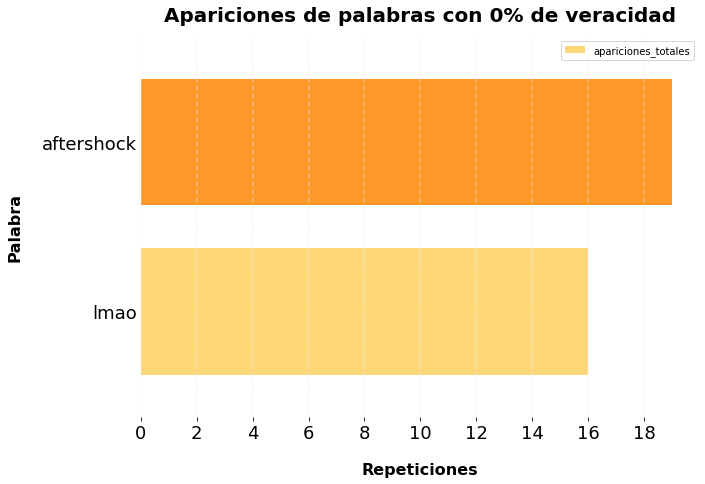
\includegraphics[width=1\textwidth]{graficos/Analisis Lexico Grafico/aparaciones_de_palabras_con_0_de_veracidad.png}
    \caption{} 
    \end{figure}
    
    De las dos palabras, una de ellas (”lmao”) es una palabra propia de una conversación  coloquial y poco seria pues significa ”Partiendose de Risa” que evidentemente no es una expresión apropiada al estar refiriéndose a un desastre.
    La otra palabra es "aftershock" su significado mas inmediato al español es réplica, el cual si esta asociado a un desastre. Que esta palabra no aparezca en ningún tweet relacionado a un desastre se puede deber a que el set de datos no es lo suficientemente grande.
    
    Análogamente al caso de las palabras con mayor veracidad, se procede a exponer las palabras que tienen menos de 10\% de veracidad en el   siguiente wordcloud :
    
     \begin{figure}[H]
    \centering
    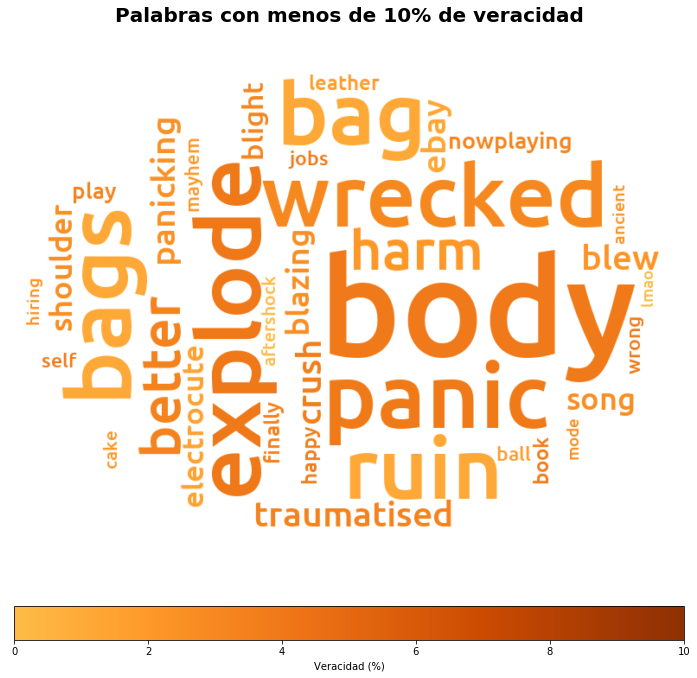
\includegraphics[width=1\textwidth]{graficos/Analisis Lexico Grafico/palabras_con_menos_de_10_de_veracidad.png}
    \caption{} 
    \end{figure}
    
    
    
    \begin{figure}[H]
    \centering
    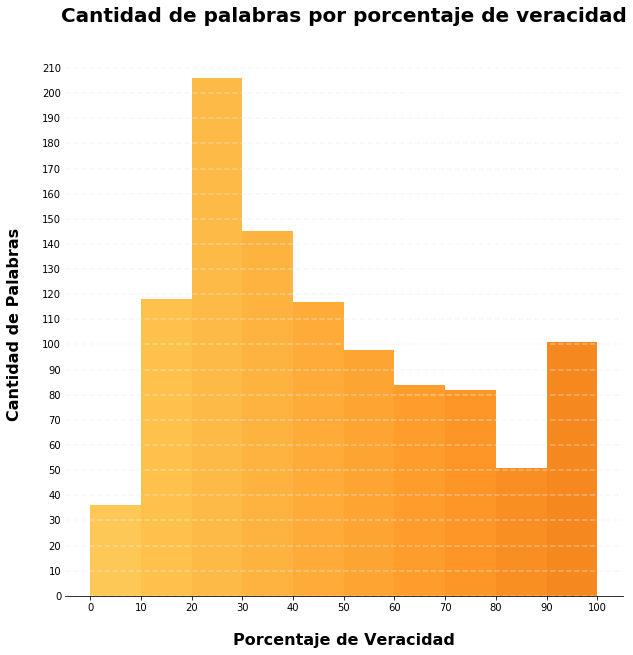
\includegraphics[width=1\textwidth]{graficos/Analisis Lexico Grafico/cantidad_de_palabras_por_porcentaje_de_veracidad.png}
    \caption{}
    \end{figure}

    La cantidad de palabras que tiene un porcentaje de veracidad elevado (mayor al 80\%), conforman una pequeña parte con respecto al total. Esto es lógico si se tiene en cuenta que la palabras con veracidad elevada son a menudo las que pertenecen al vocabulario o familia de palabras empleadas cuando se busca hablar o dar información acerca de un accidente o desastre. El pico que se observa para valores entre  20\% y  40\% puede deberse al uso de un lenguaje mas informal que predomina en la red social y que si bien puede tratar sobre desastres también es la forma usual de comunicación de una importante cantidad de usuarios de la plataforma, y al set de datos tener mas tweets que "falsos" es esperable que dicho este en un punto mas bajo que el 50\%. 
    
    Con el objetivo de extraer mayores conclusiones, se puede agregar una variable más al estudio de la veracidad, tal como la prolongación de los Tweets tanto en palabras como caracteres. De esta manera, se elaboraron las siguientes visualizaciones.

    \begin{figure}[H]
    \centering
    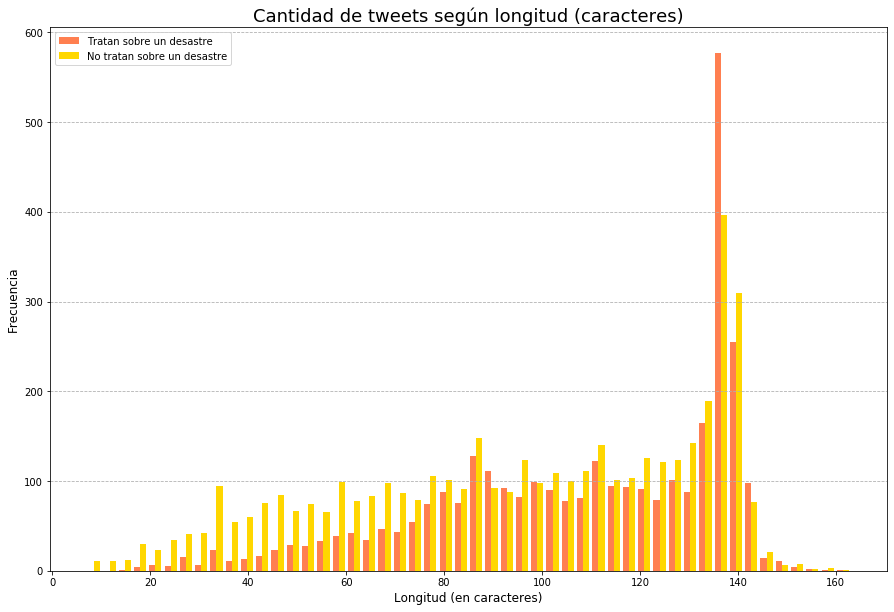
\includegraphics[width=1\textwidth]{graficos/Analisis Lexico Grafico/cantidad_de_tweets_segun_longitud_en_caracteres.png}
    \caption{}
    \end{figure}
    
    Como se puede observar, hay una marcada diferencia en la distribución de los Tweets según su longitud en caracteres. Se observa que los Tweets que efectivamente refieren a desastres tienden a ser mas largos que los que no. Esto puede deberse a que las personas que escriben estos Tweets tienden a querer aportar la mayor cantidad de información posible sobre el mismo, con una considerada cantidad de detalles. Con lo cual seria lógico que estos resulten ser mas extensos.
    
    Por otro el otro lado, se observa que dentro de los tweets de menor cantidad de caracteres suelen prevalecer los falsos. Esto es esperable siguiendo el razonamiento previamente explicado.
    
    
    Algo que puede ser de interés es analizar la veracidad de los tweets según la cantidad de palabras que contienen.
    
    \begin{figure}[H]
    \centering
    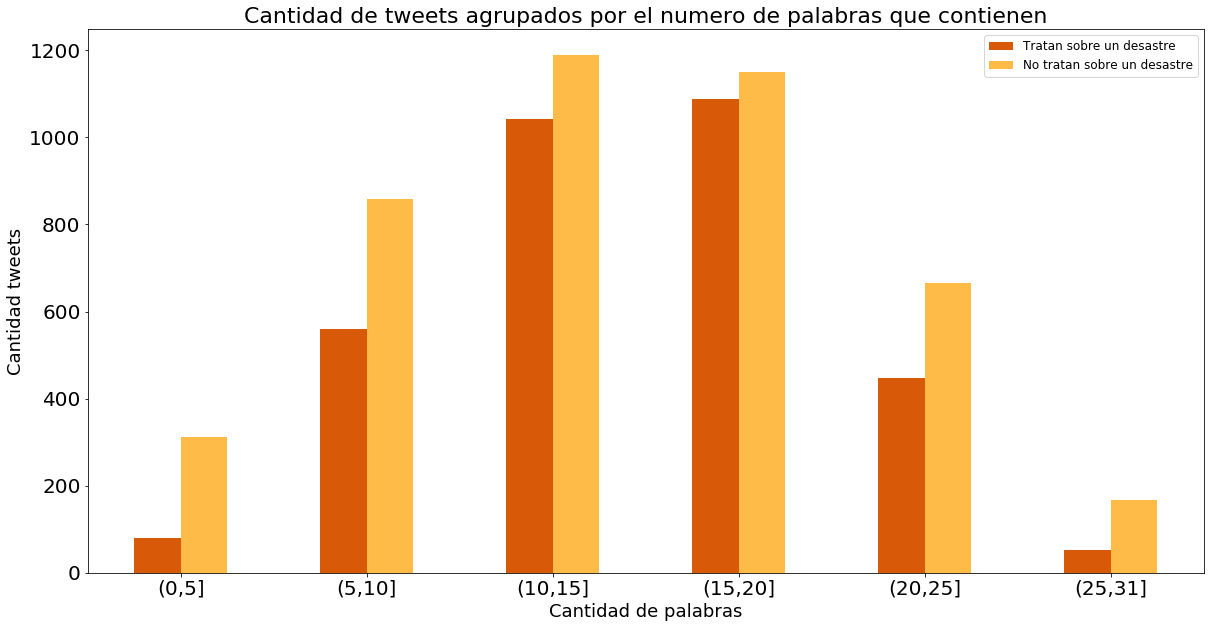
\includegraphics[width=1\textwidth]{graficos/Analisis Lexico Grafico/cantidad_de_tweets_agrupados_por_numero_de_palabras.png}
    \caption{}
    \end{figure}
    
    El gráfico muestra que sin importar el grupo, la cantidad de Tweets que no tratan sobre una tragedia es mayor que la de Tweets que si lo hacen. Además no se pueden observar esos intervalos tan claros donde hay una gran diferencia entre tweets que tratan sobre el target y los que no. En base a esto y que en el grafico de caracteres si se puede observar una diferencia, podemos inferir que los tweets veraces tienden a usar palabras mas largas.
    
    Graficamos la longitud promedio de las palabras según a que tipo de tweet pertenecen. 
    
     \begin{figure}[H]
    \centering
    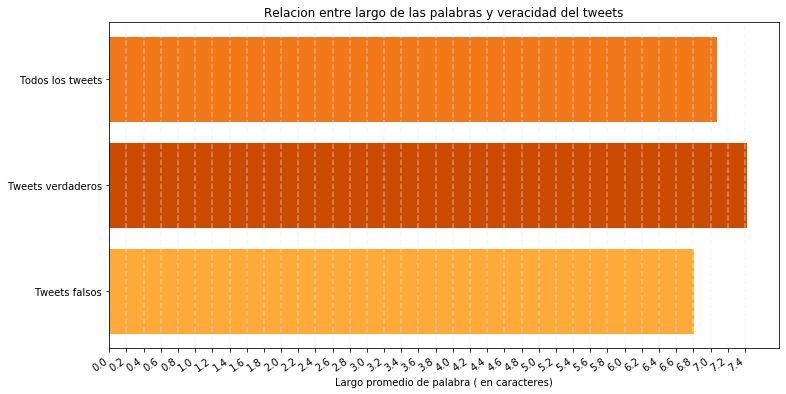
\includegraphics[width=1\textwidth]{graficos/Analisis Lexico Grafico/longitud promedio barras.png}
    \caption{}
    \end{figure}

    En este gráfico se puede observar efectivamente que los tweets veraces tienden a tener palabras mas largas, lo cual confirma nuestra hipotesis previa.

    
    Finalmente, debido a que Twitter es una red social que posee características propias con funcionalidades tales como '\#' o '@', se procedió a hacer un análisis de la relación existente entre la aparición estos caracteres específicos dentro de un Tweet y la veracidad del mismo. Además, se agrega a este estudio la consideración de la existencia de símbolos lingüísticos usuales (¡, !, ¿, ?), nombres de locaciones geográficas, direccionamientos a páginas web (URLs) o el simple hecho de que el Tweet comience con letra mayúscula, puesto que son casos particularmente interesantes de analizar en caso de que exista alguna tendencia.

    \begin{figure}[H]
    \centering
    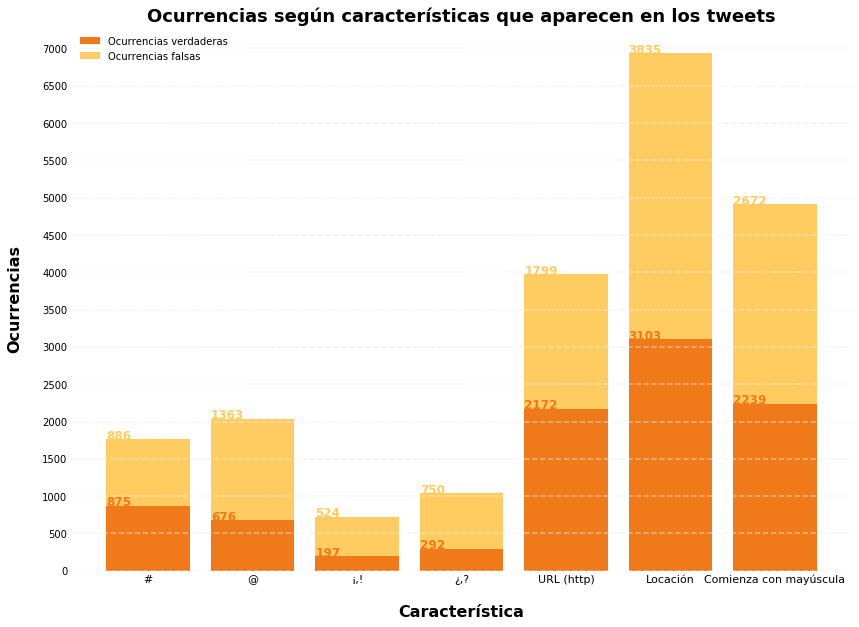
\includegraphics[width=1\textwidth]{graficos/Analisis Lexico Grafico/ocurrencias_segun_caracteristicas_que_aparecen_en_los_tweets.png}
    \caption{} 
    \end{figure}
    
    Al examinar los resultados obtenidos se puede afirmar que la presencia de '\#', URLs, locaciones y mayúsculas como letra inicial no posee impacto en la veracidad de los Tweets. Caso contrario es el observable en aquellos que incluyen signos de exclamación, interrogración y '@' en su contenido, puesto que sólo alrededor de un tercio (27.3\%, 28\% y 33.2\%, respectivamente) de los Tweets que contienen alguno de estos caracteres tratan sobre desastres reales. Esto se puede deber a que los medios formales de comunicación no utilizan estos caracteres para comunicar información sobre desastres.
    
    Por otra parte, otro de los aspectos que se puede analizar frente a la presencia de estas características específicas es el de la longitud de los Tweets que las poseen. Los siguientes dos gráficos representan los resultados obtenidos con dicho afán.

    \begin{figure}[H]
    \centering
    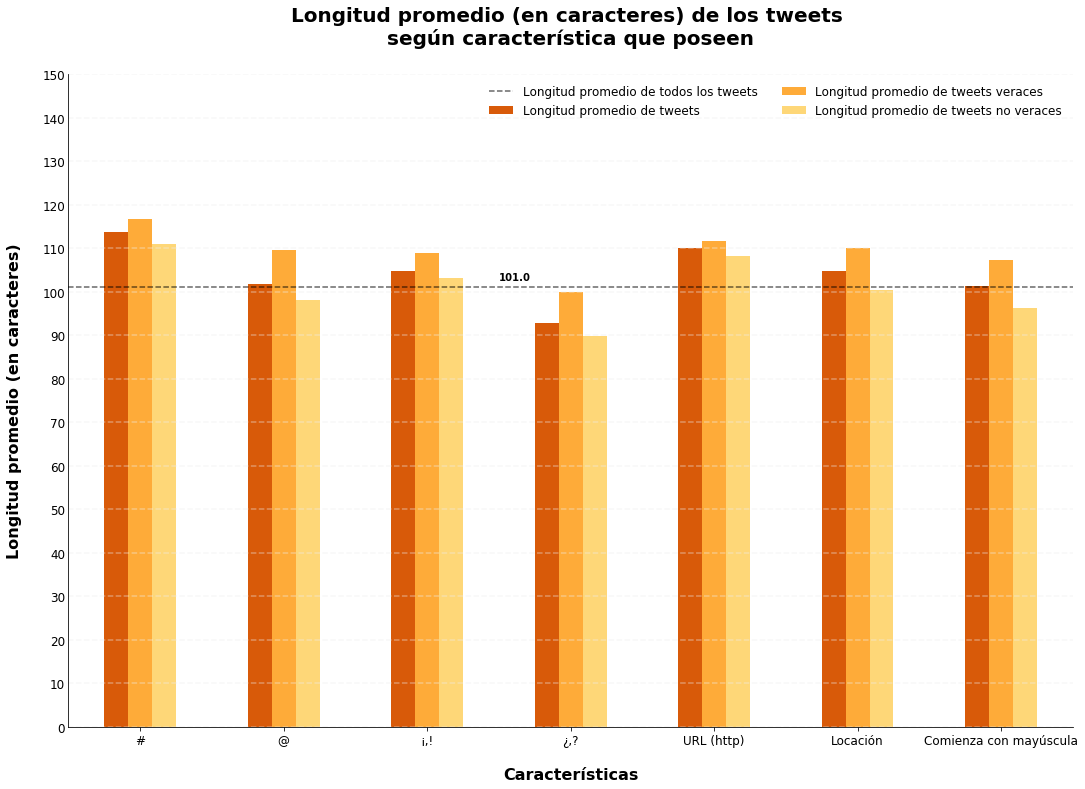
\includegraphics[width=1\textwidth]{graficos/Analisis Lexico Grafico/long_promedio_char_tweets_segun_caracteristica.png}
    \caption{} 
    \end{figure}
    
    \begin{figure}[H]
    \centering
    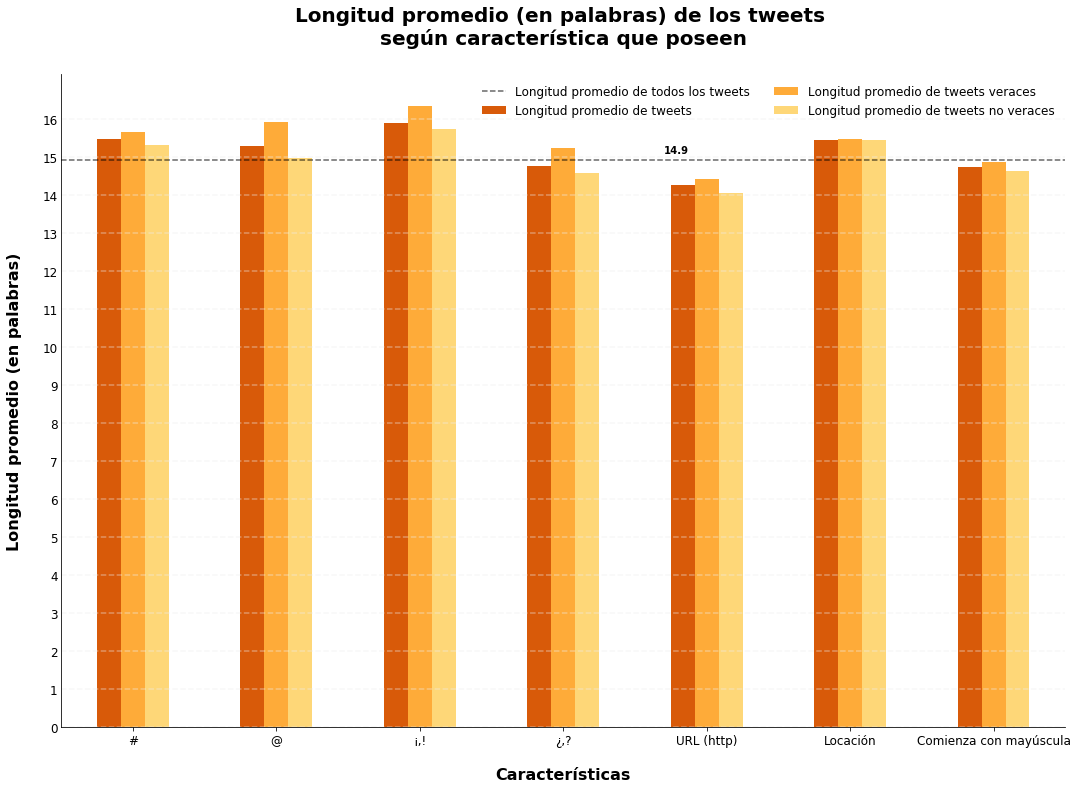
\includegraphics[width=1\textwidth]{graficos/Analisis Lexico Grafico/long_prom_words_tweets_segun_caracteristicas.png}
    \caption{} 
    \end{figure}
    
    A partir de estas visualizaciones se puede observar una serie de leves tendencias. La primera es que la prolongación promedio de los Tweets veraces posee una inclinación a ser mayor a la de los Tweets que no tratan sobre desastre, ya sea en caracteres o palabras, sin importar la característica que posean.
    
    Por otro lado, la longitud en caracteres de aquellos Tweets que contienen signos de interrogación es menor al promedio, al igual que la extensión en palabras de aquellos Tweets que contienen direcciones de enlace (URLs). 
    
    Es notable que los Tweets que poseen locación tienen la misma longitud promedio independientemente de su veracidad y esta se encuentra ligeramente sobre el promedio.  
    
    \newpage
    \section{Análisis de Keyword}\label{sec:intro}

    Se continúa con el análisis de las Keywords usadas en los Tweets. Es relevante aclarar que para los análisis que prosiguen no se tendrán en cuenta todas las Keywords, sólo se consideran aquellas que se encuentran asociadas a 29 o más Tweets. Esta decisión es tomada para evitar el problema de la sobrerepresentación de aquellas cuya cantidad de repeticiones es inferior en comparación al resto. 
    
    Para ello, en primer instancia se calcula el promedio de repetición de las 222 distintas Keywords (a los Tweets que no poseen Keyword asociada, se les asigna 'none\_keyword'), obteniendo como resultado alrededor de 34 repeticiones por Keyword. Sin embargo, recortar el espectro estudiado en este valor significa dejar fuera del análisis a alrededor del 35\% (77 Keywords) del total, por ello se opta por reducir la vara a 29, donde sólo 13 de ellas no son tenidas en cuenta y la distancia al valor promedio no es significativa. 
    
    Para comenzar se pretende estudiar la relación entre el uso de las distintas Keywords con la prolongación del texto de los Tweets asociados a ellas. Este primer gráfico muestra la longitud promedio de los Tweets agrupados por Keyword. 

    \begin{figure}[H]
    \centering
    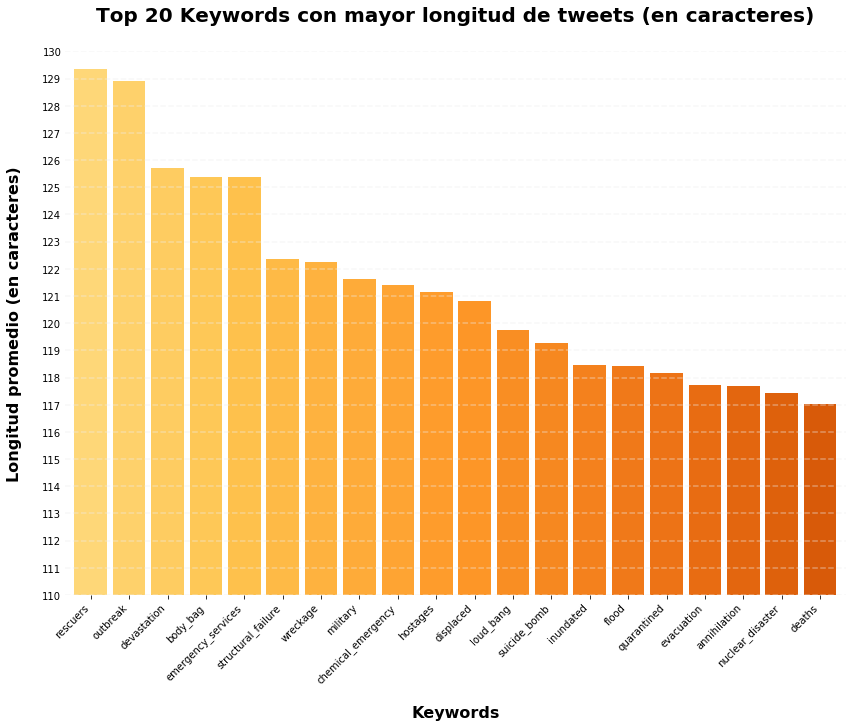
\includegraphics[width=1\textwidth]{graficos/Analisis de Keyword/top_20_long_con_mayor_long_de_tweets.png}
    \caption{} 
    \end{figure}
    
    Como se puede apreciar, las longitudes se acercan al límite de 140 caracteres por Tweet que ofrece la plataforma, pues más de la mitad se encuentran sobre los 120 caracteres. 
    
    Si ahora realizamos el mismo análisis modificando la manera en que se mide la longitud a palabras por Tweet, se obtiene el siguiente gráfico:
    
    \begin{figure}[H]
    \centering
    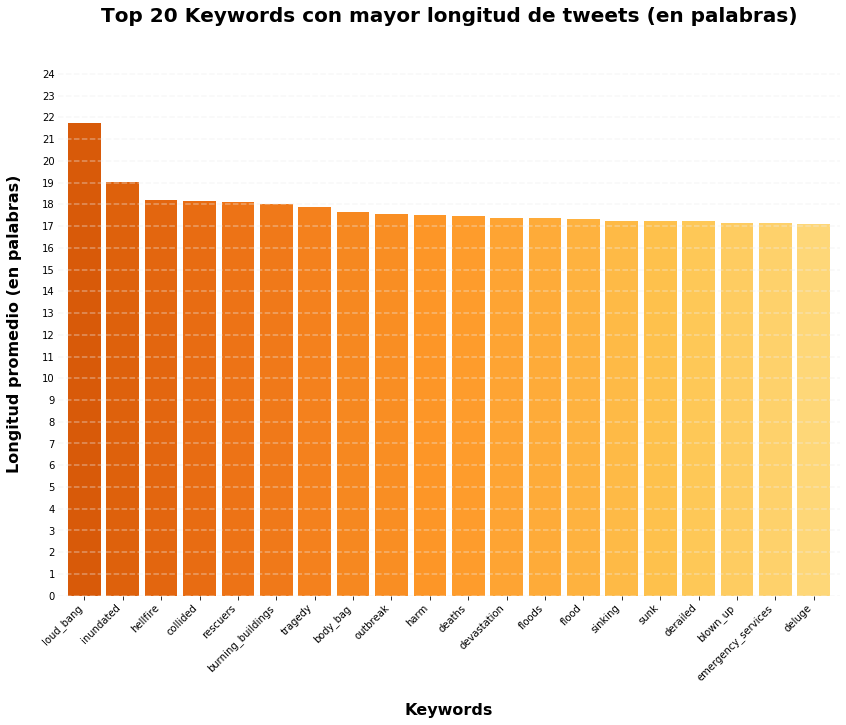
\includegraphics[width=1\textwidth]{graficos/Analisis de Keyword/top_20_keywords_con_mayor_long_de_tweets_en_palabras.png}
    \caption{} 
    \end{figure}
     
    Se puede observar que la mayoría de Keywords corresponden a Tweets que tienen como media entre 17 y 18 palabras.
    
    De forma análoga, se estudian las Keywords que corresponden a Tweets con menor longitud promedio en caracteres. 
    
    \begin{figure}[H]
    \centering
    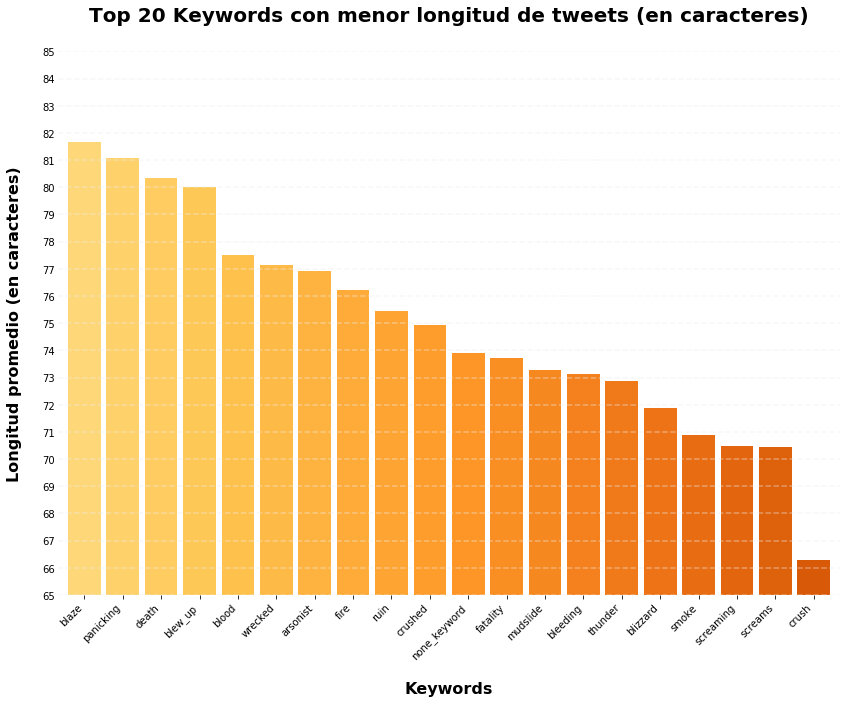
\includegraphics[width=1\textwidth]{graficos/Analisis de Keyword/top_20_keywords_con_menor_long_de_tweets_en_caracteres.png}
    \caption{} 
    \end{figure}
    
    Se puede observar claramente que la longitud promedio mínima con diferencia esta sobre los 66 caracteres. Además, comparado con las Keywords con mayor longitud en caracteres, hay una diferencia notable. 
    
    Ahora, midiendo la longitud en palabras, se obtiene el siguiente gráfico:
    \begin{figure}[H]
    \centering
    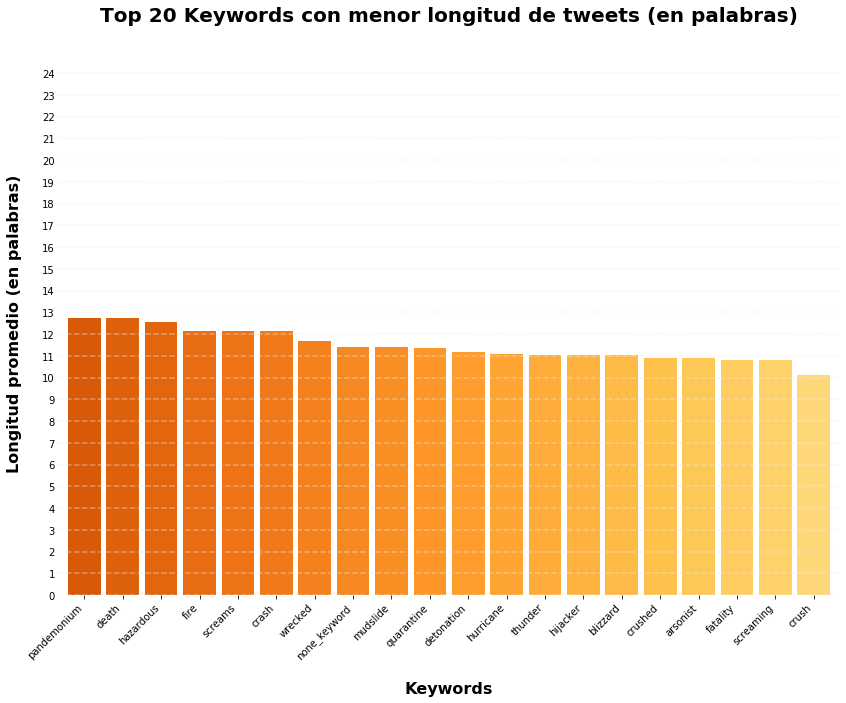
\includegraphics[width=1\textwidth]{graficos/Analisis de Keyword/top_20_keywords_con_menor_long_de_tweets.png}
    \caption{} 
    \end{figure}
    Se observa que la longitud promedio mínima esta sobre las 10 palabras. Se observa que comparado con las Keywords con mayor longitud en palabras, la diferencia de longitudes no es significativa. 
    
    Como conclusión de las últimas visualizaciones se puede establecer firmemente que no existe ninguna relación aparente entre la prolongación del Tweet y la Keyword asociada a este. Esto se debe a que ninguno de los grupos de Keywords representadas en cada gráfico presentan rasgos que los distingan del resto, todos se relacionan a algún tipo de desastre (sin importar la naturaleza del mismo).
    
    De manera análoga a la sección anterior, el mayor interés del análisis exploratorio relacionado con las Keywords llega cuando se agrega al estudio el porcentaje de veracidad del total de Tweets asociados a un mismo Keyword.    
    
    Como visualización inicial se procede a mostrar aquellos Keywords asociados a los grupos de Tweets con mayor grado de veracidad.
    
    \begin{figure}[H]
    \centering
    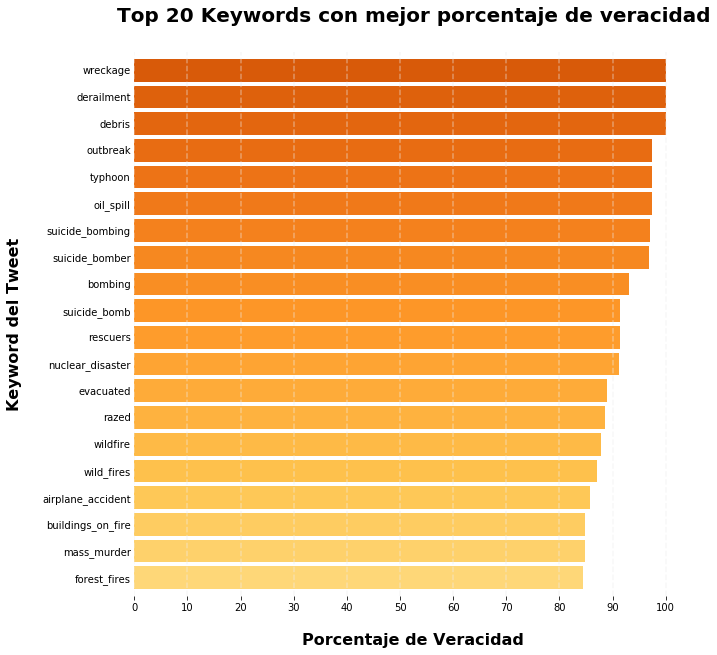
\includegraphics[width=1\textwidth]{graficos/Analisis de Keyword/top_10_keywords_con_mejor_porcentaje_de_veracidad.png}
    \caption{} 
    \end{figure}
    
    Como se observa, gran parte de las Keywords pertenecen o tienen una relación estrecha con el conjunto/familia de palabras que son empleadas a menudo para describir o dar información acerca de accidentes o desastres. Asimismo muchas de estas difícilmente podrían ser empleadas en cualquier otro tipo de contexto o situación, y es muy probablemente por esa razón que presentan tan elevada veracidad. Tal es el caso de palabras como ''derailment'', la cual significa descarrilamiento, o ''debris'', escombros. Ambas Keywords se encuentran entre las de mayor veracidad y sus significados pueden ser considerados muy puntuales, corroborando la explicación anterior. 
    
    En contraposición a estas Keywords se hallan aquellas cuya veracidad asociada es extremadamente pequeña y, a los fines de demostrar claramente las diferencias entre ambos casos, se enseñan a continuación preservando la escala de la última visualización.
    
    \begin{figure}[H]
    \centering
    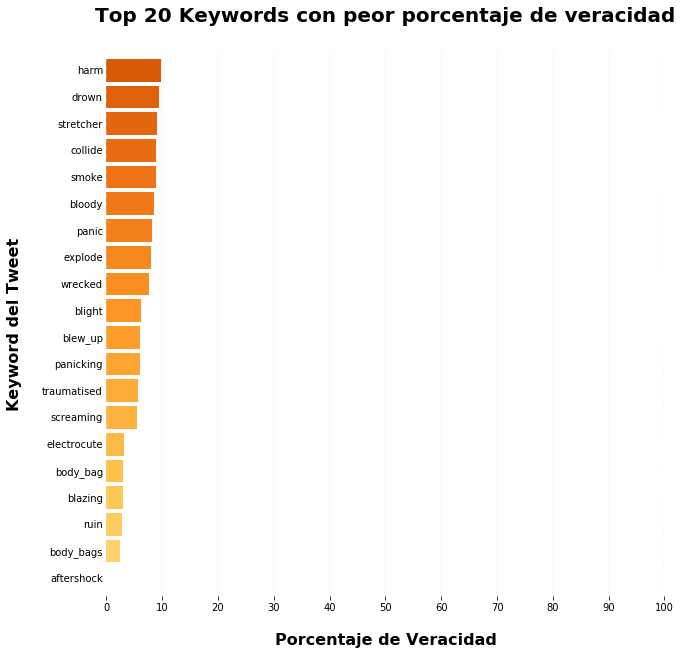
\includegraphics[width=1\textwidth]{graficos/Analisis de Keyword/top_20_keywords_con_peor_porcentaje_de_veracidad.png}
    \caption{} 
    \end{figure}
    
    A diferencia del anterior gráfico, estas Keywords no pueden ser consideradas ''exclusivas'' del conjunto de palabras frecuentemente utilizadas para referirse a desastres/accidentes. Son palabras de las cuales se puede hacer uso en contextos muy diversos completamente diferentes a los concernientes a este trabajo y es por esa razón que tienen tan baja veracidad (<10\%). Por ejemplo, ''smoke'' significa humo, ''ruin'' se traduce como ruina y ''screaming'',gritando. Estas tres palabras pueden ser utilizadas en diversos ámbitos para múltiples situaciones.
    
    Si bien ahora se conocen las Keywords con mayor y menor grado de veracidad, resulta atractivo poder visualizar cuáles de ellas se encuentran entre las de mayor y menor cantidad de Tweets asociados. Para lograr esto, en primer lugar se grafican las 10 Keywords con mayor y con menor frecuencia de aparición.
    \begin{figure}[H]
    \centering
    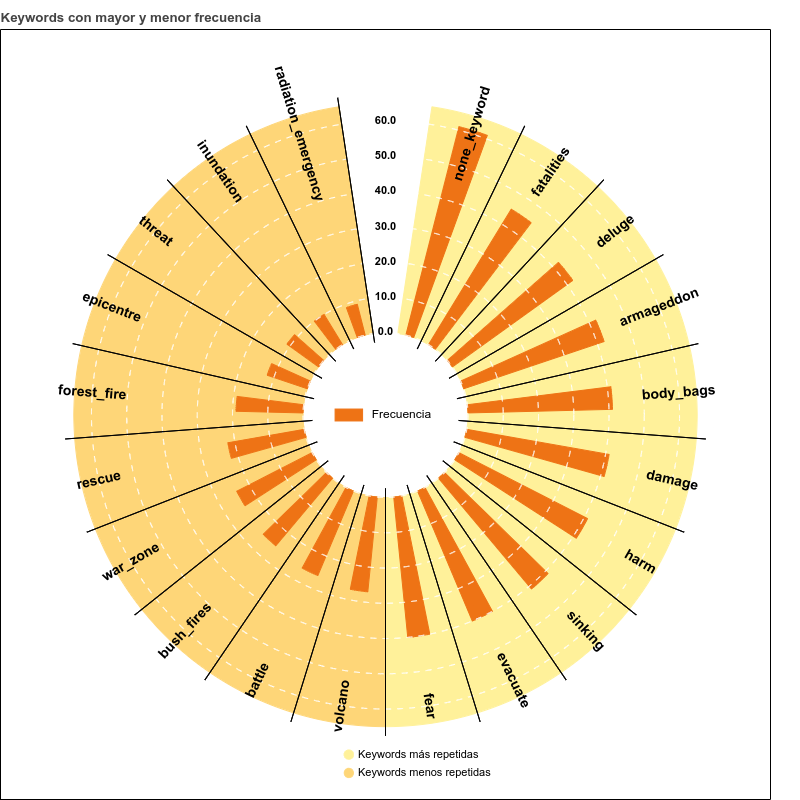
\includegraphics[width=1\textwidth]{graficos/Analisis de Keyword/rosquete_keywords_repetidas.png}
    \caption{} 
    \end{figure}
    
    A partir de esta información se puede proceder a vincular los datos sobre veracidad asociada a un Keyword y la cantidad que veces que aparece. El producto de esto se ve representado en la wordcloud que se enseña a continuación. Cabe destacar que, de igual manera que en los anteriores gráficos de este estilo, cuanto mayor sea la frecuencia de una palabra, mayor será el tamaño de esta en la visualización.
    
    \begin{figure}[H]
    \centering
    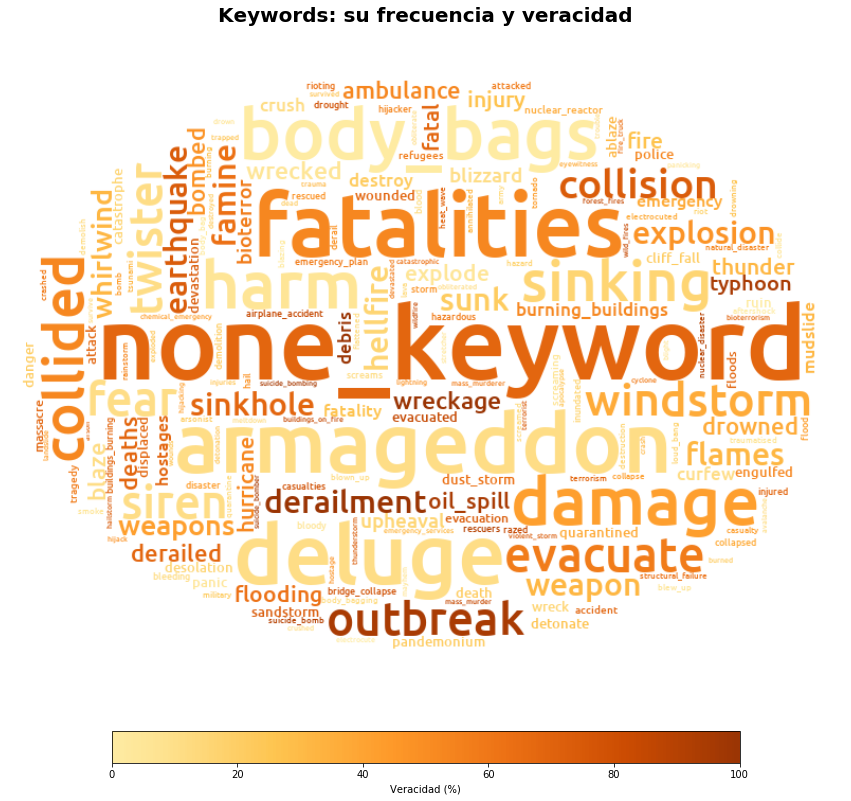
\includegraphics[width=1\textwidth]{graficos/Analisis de Keyword/keywords_frec_y_veracidad.png}
    \caption{} 
    \end{figure}
    
    Por medio de este gráfico se puede apreciar que una gran cantidad de Tweets no tienen una Keyword asociada y que, además, éstos tienen un alto porcentaje de veracidad. Otras Keywords destacables debido a su cantidad y porcentaje de veracidad son: ``outbreak'', ''collision'', ``fatalities'' y ``damage'', lo cual tiene sentido ya que son palabras que se usan a menudo cuando se quiere hacer referencia a accidentes. 
    
    También cabe destacar que a pesar de tener Tweets de varias partes del mundo, todas éstas Keywords se encuentran en inglés, pero esto puede deberse a que el set de datos utilizado está conformado en su gran mayoría por Tweets en ese idioma.
    
    \begin{figure}[H]
    \centering
    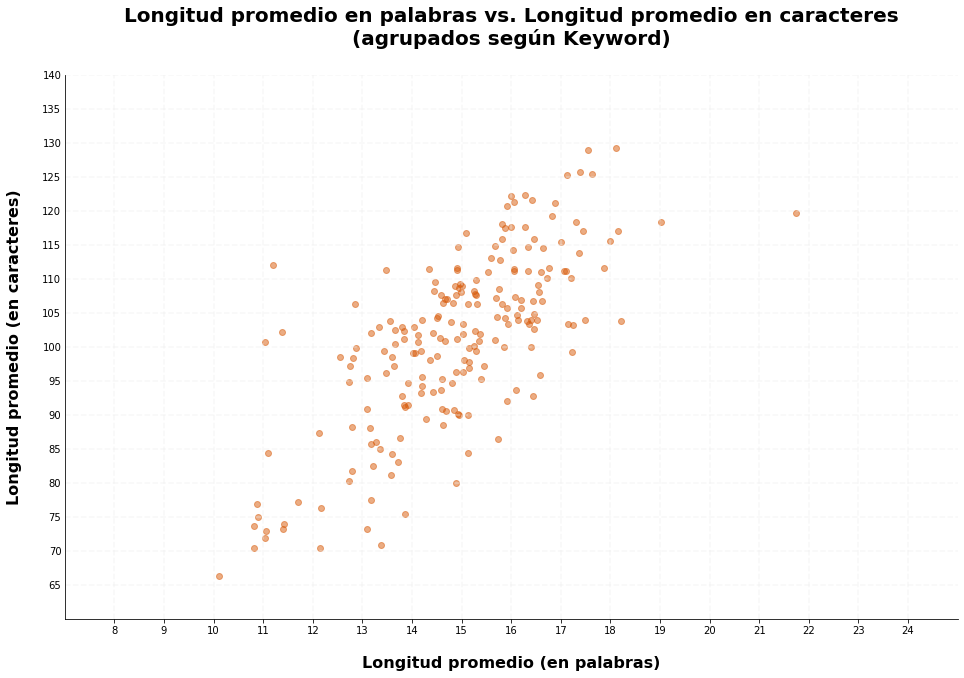
\includegraphics[width=1\textwidth]{graficos/Analisis de Keyword/long_prom_en_palabras_vs_long_prom_en_Caracteres.png}
    \caption{} 
    \end{figure}
    
    
    \begin{figure}[H]
    \centering
    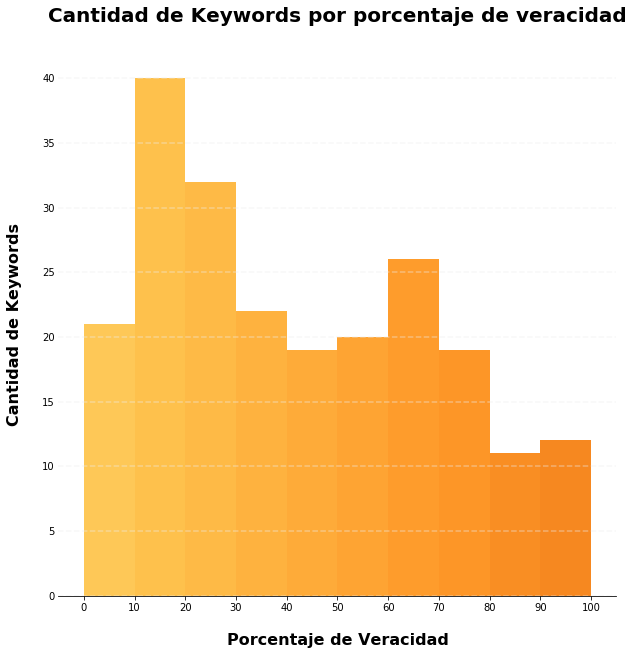
\includegraphics[width=1\textwidth]{graficos/Analisis de Keyword/cantidad_de_keywords_por_porcentaje_de_veracidad.png}
    \caption{} 
    \end{figure}
    
    Se puede apreciar que después del pico que se da entre el 10 y 20\% de veracidad donde llega a 40 Keywords, la cantidad de Keywords bajando casi constantemente. Se puede concluir que los Tweets bajo porcentaje de veracidad tienden a usar mas Keywords que aquellos con un alto porcentaje de veracidad.
    
    \begin{figure}[H]
    \centering
    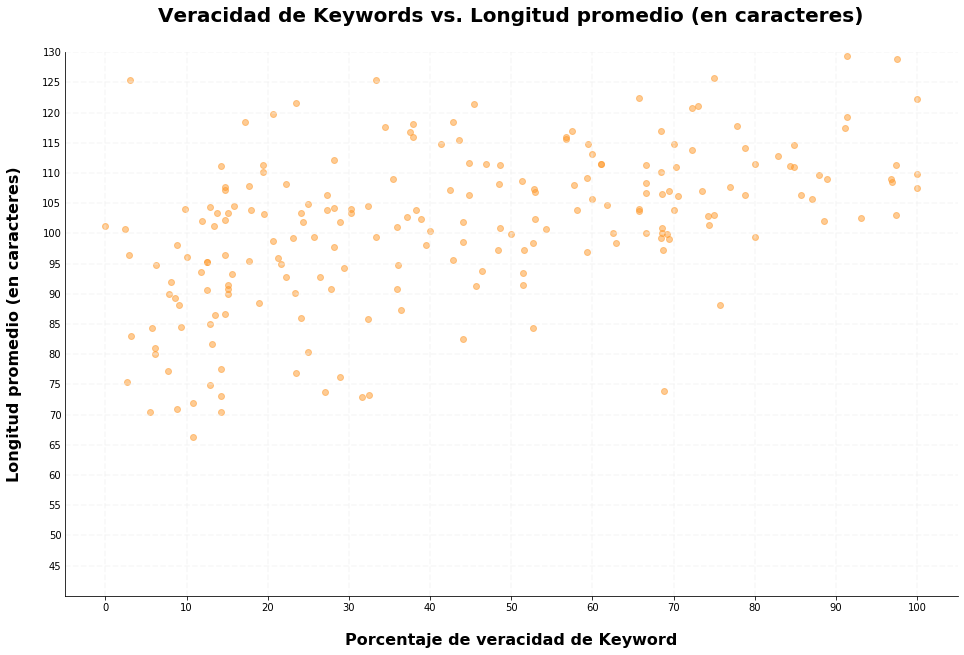
\includegraphics[width=1\textwidth]{graficos/Analisis de Keyword/veracidad_keywords_vs_long_promedio_en_caracteres.png}
    \caption{} 
    \end{figure}
    
    Se puede observar una relación que puede ser considerada como lineal
    
    Los Keywords que tienen menor veracidad tienden a hacer referencia a Tweets de menor longitud
    
    \begin{figure}[H]
    \centering
    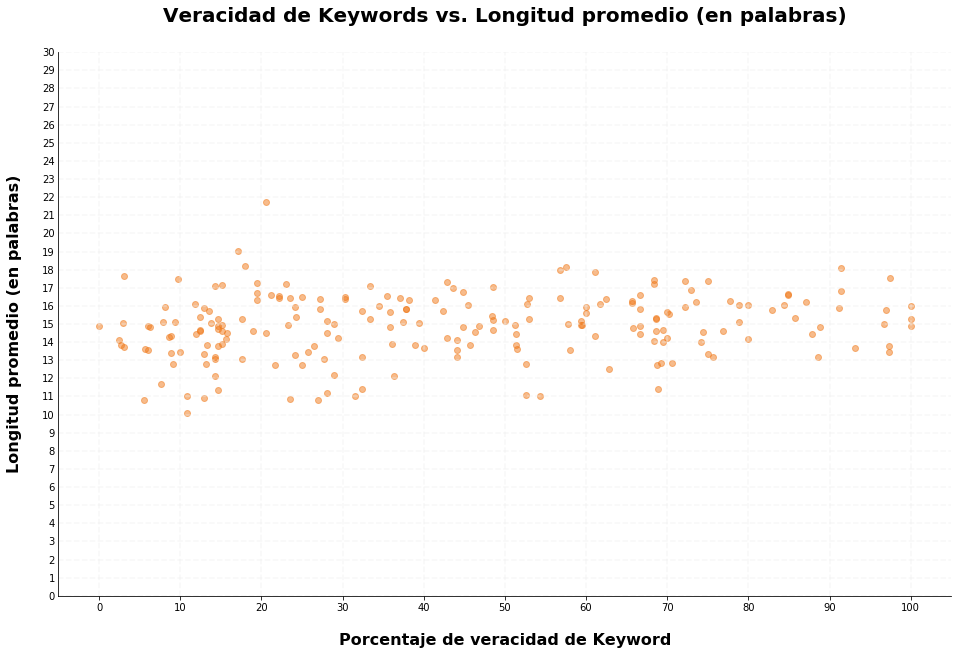
\includegraphics[width=1\textwidth]{graficos/Analisis de Keyword/veracidad_de_keywords_vs_long_promedio_en_palabras.png}
    \caption{} 
    \end{figure}
    
    La distribución de las Keywords puede considerarse uniforme respecto de su veracidad, aunque puede observarse una concentración ligeramente mayor para los valores de veracidad mas bajos
    
    \newpage
    
    Los siguientes gráficos resumen la relación que hay tanto entre las Keywords mas veraces como las menos veraces con la longitud tanto en caracteres como en palabras de los Tweets asociados
    
    \begin{figure}[H]
    \centering
    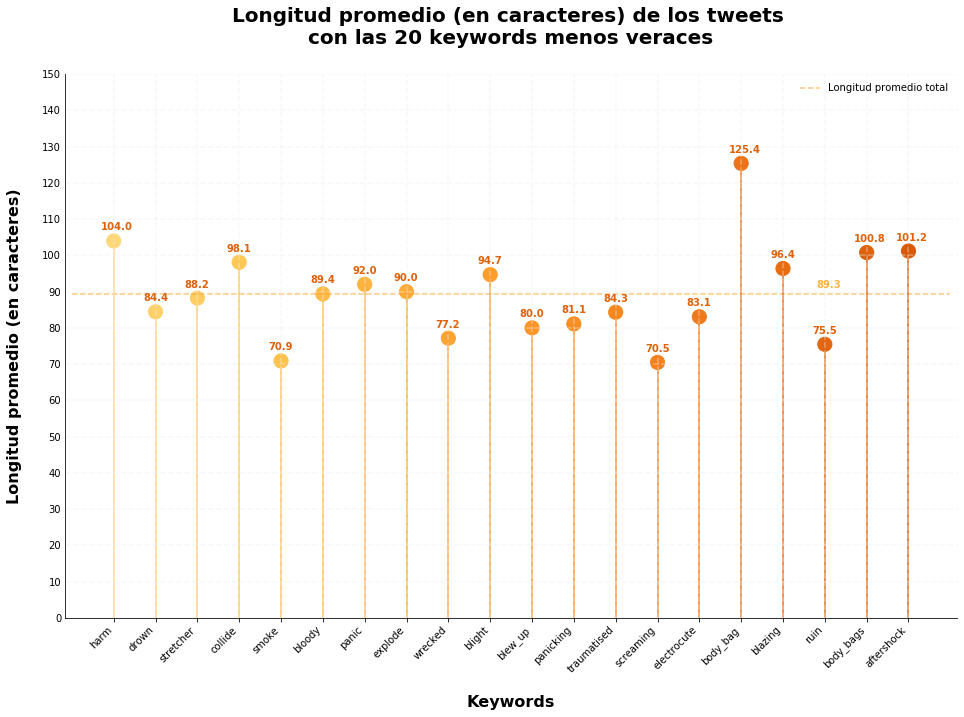
\includegraphics[width=1\textwidth]{graficos/Analisis de Keyword/long_prom_char_keywords_no_veraces.png}
    \caption{} 
    \end{figure}
    
    Se puede observar que la longitud promedio en caracteres de los Tweets asociados a las 20 Keywords menos veraces esta ligeramente por encima de los 89 caracteres (89,3). También se puede ver a simple vista que la Keyword ''body\_bag'' que significa ''bolsa para cadáveres'' aunque en ciertos contextos puede interpretarse como un tipo de ''bolso'' o ''cartera'' tiene asociados Tweets mas largos con diferencia respecto a las demás, con una longitud promedio de 125 palabras aproximadamente (125,4) 
    
    \begin{figure}[H]
    \centering
    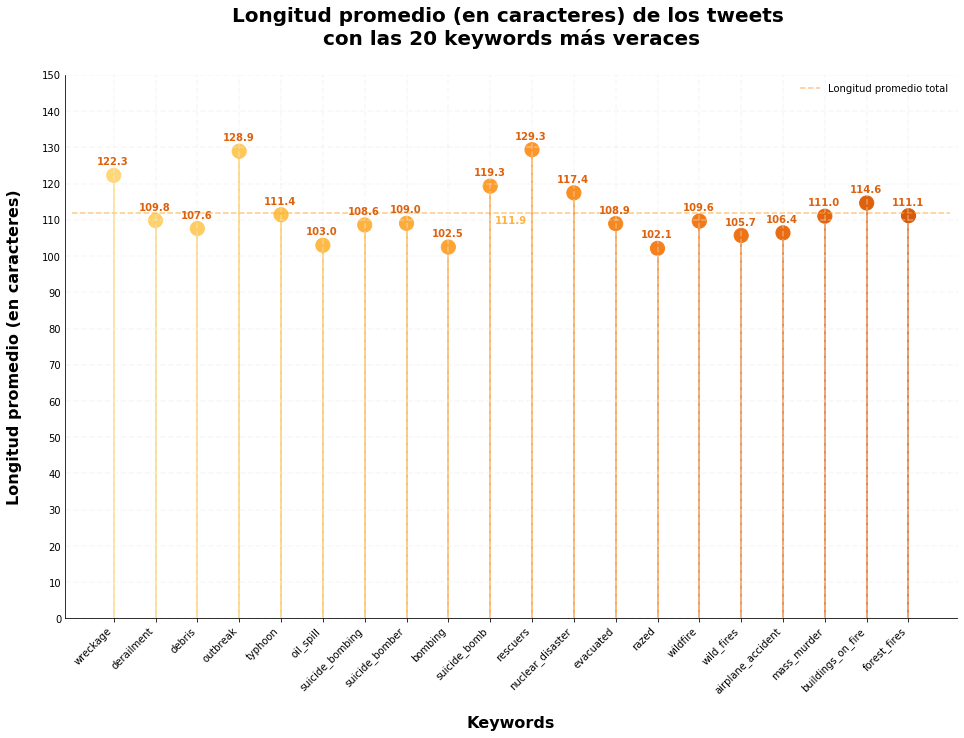
\includegraphics[width=1\textwidth]{graficos/Analisis de Keyword/long_prom_char_keywords_veraces.png}
    \caption{} 
    \end{figure}
    
    Se puede apreciar que todas las longitudes promedio de los Tweets asociados a las 20 Keywords mas veraces están todas sobre los 100 caracteres y no presentan tanta dispersión como el gráfico anterior. En promedio estas tienen una longitud aproximada de 112 palabras (111,9). También se puede ver a simple vista que los valores de las Keywords ''rescuers'' que significa ''rescatadores'' y ''outbreak'' que significa ''brote'' destacan sobre el resto por tener una longitud de Tweets ascociados levemente mayor al resto  
    
    Una observación importante muy fácil de ver es que los Tweets que tienen asociadas Keywords mas veraces tienden a ser considerablemente mas largos que los que tienen una Keyword poco veraz. La diferencia promedio es de 111,9 - 89,3 = 22,6; Esto puede deberse a que las ''Kewords más veraces'', tienen asociados un mayor porcentaje de Tweets que efectivamente hacen referencia a desastres/accidentes que las ''Keywords menos veraces'' y como se vio anteriormente la longitud en caracteres de los Tweets veraces es mayor a la de los falsos.
    
    \newpage
    Análogamente, se procede a estudiar que ocurre con la longitud promedio en palabras de los Tweets asociados a las Keywords que presentan menor y mayor porcentaje de veracidad.
    
    \begin{figure}[H]
    \centering
    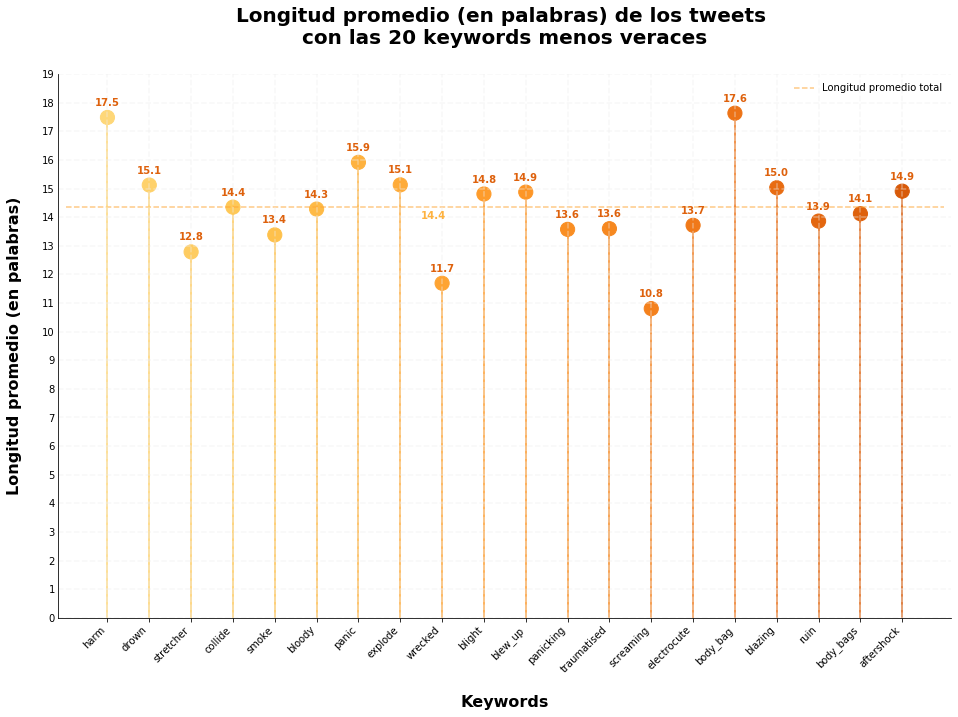
\includegraphics[width=1\textwidth]{graficos/Analisis de Keyword/long_prom_words_keywords_no_veraces.png}
    \caption{} 
    \end{figure}
    
    Se puede apreciar que la longitud promedio es de aproximadamente 14 palabras (14,4). También se puede ver a simple vista que los valores de las Keywords ''body\_bag'' y ''harm'' que significa ''daño'' destacan sobre el resto por tener Tweets asociados con una longitud en palabras levemente mayor al resto.
     
    
    \begin{figure}[H]
    \centering
    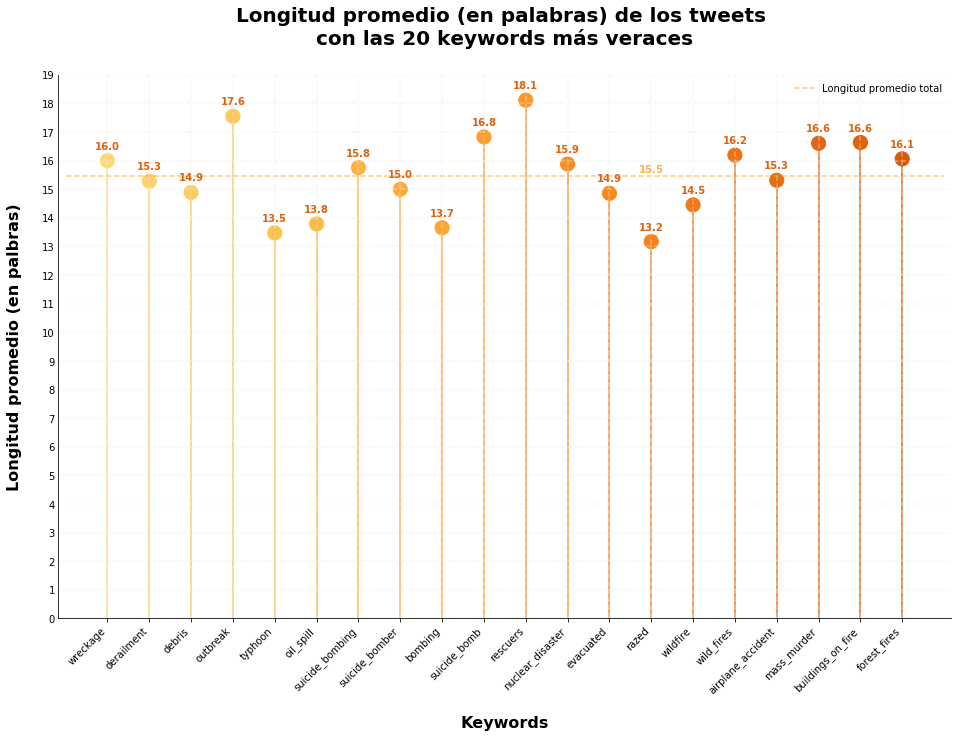
\includegraphics[width=1\textwidth]{graficos/Analisis de Keyword/long_prom_words_keywords_veraces.png}
    \caption{} 
    \end{figure}

    En comparación con la longitud promedio en palabras de los Tweets asociados a Keywords menos veraces, se nota una dispersión de los datos sutilmente menor. También se puede apreciar que la longitud promedio es próxima a 15 palabras (15,5). Con lo cual podemos llegar a la conclusión de que la diferencia en el promedio es de 15,5 - 14,4 = 1,1.
    
    La diferencia entre la longitud en palabras de los Tweets asociados a las Keywords mas veraces con respecto a los asociados a las Keywords menos veraces es en promedio de 1 palabra (1,1). Esta es una diferencia marcada pero no tan sustancial como en el análisis de la Longitud en caracteres. Resultado que corrobora lo expuesto anteriormente.
    
    \begin{figure}[H]
    \centering
    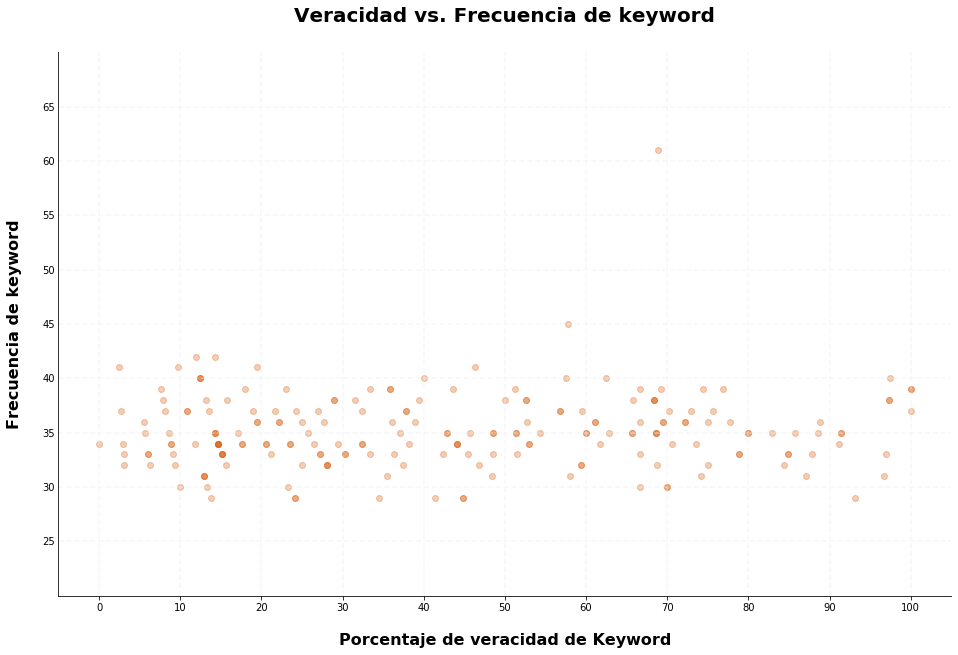
\includegraphics[width=1\textwidth]{graficos/Analisis de Keyword/veracidad_vs_frec_de_keyword.png}
    \caption{} 
    \end{figure}
    
    En el siguiente gráfico se muestran las Keywords más usadas en un mayor tamaño y las menos usadas en menor tamaño. Por otro lado, el color hace referencia a la veracidad promedio. Para los Tweets en los que no se especificaba una Keyword, se tomo el valor "none\_keyword". A pesar de mostrar los datos de forma cualitativa en lugar de cuantitativa, el gráfico da una ida de cuales son las Keywords más usadas y cuales son las más verídicas. 
    
    Los siguientes 2 gráficos exponen la anterior WordCloud de manera más cuantitativa.
    
    
    
    \newpage
    \section{Análisis de Locación}\label{sec:intro}
    
    Analizando la cantidad de Tweets que tienen una ubicación especificada con respecto a los que no, se llega a la información expresada en el siguiente gráfico. La gran mayoría de Tweets tienen una locación especificada (66,7\%).
    
    \begin{figure}[H]
    \centering
    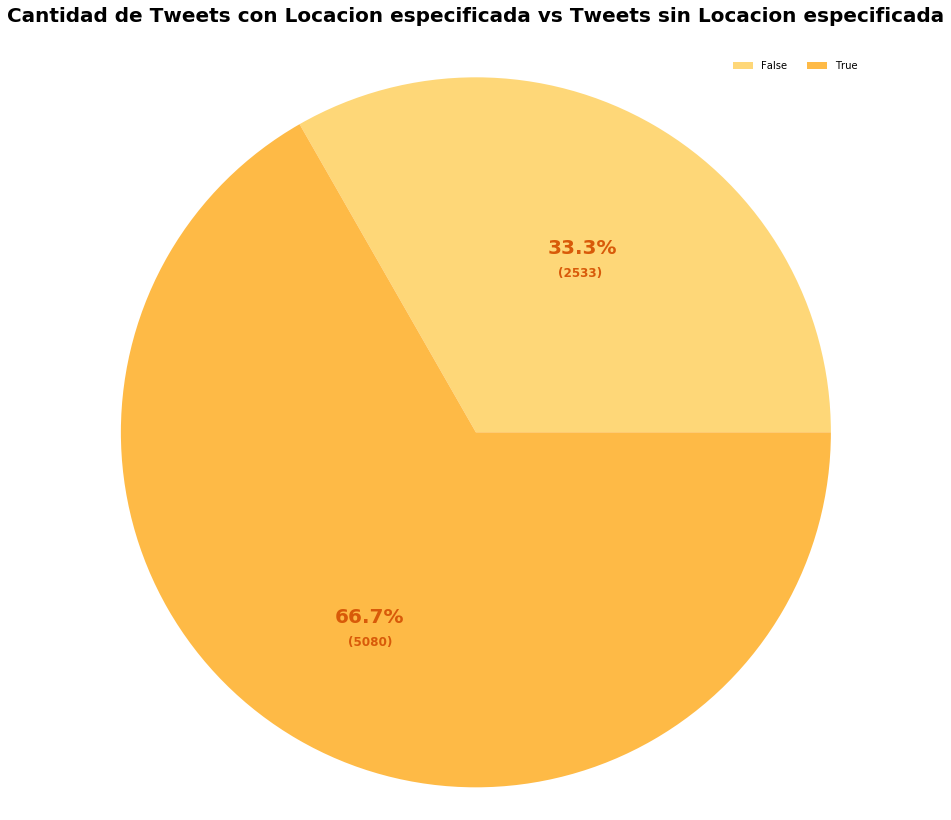
\includegraphics[width=1.1\textwidth]{graficos/Analisis de Locacion/cantidad_de_tweets_con_locacion_especificada_vs_sin_locacion_especificada.png}
    \caption{} 
    \end{figure}
    
    Si contamos la cantidad de apariciones que tiene cada ''Location'' sin tener en cuenta aquellos Tweets en los que este campo no esta especificado debido a que son considerablemente mas que los Tweets cualquier otra locación, con lo cual quedaba sobredimensionado en el gráfico en comparación del resto y por eso se decidió no incluirla.
    
    \begin{figure}[H]
    \centering
    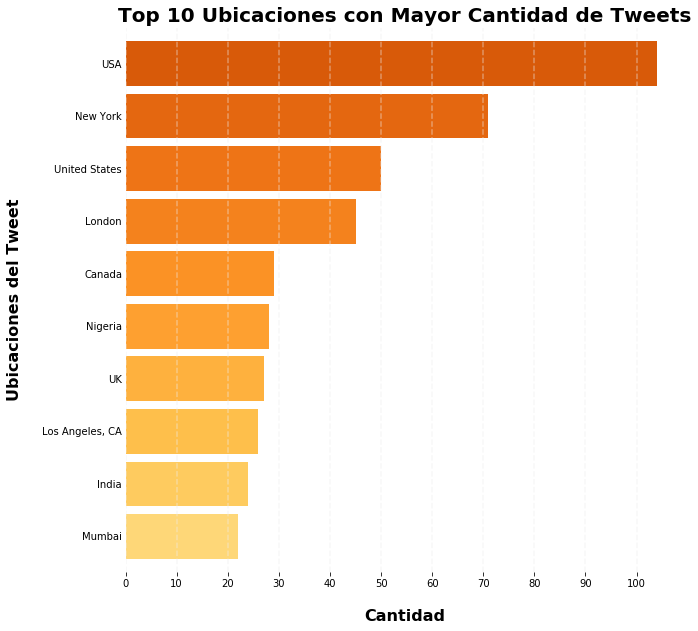
\includegraphics[width=1.1\textwidth]{graficos/Analisis de Locacion/top_10_locaciones_con_mayor_cantidad_de_tweets.png}
    \caption{} 
    \end{figure}
    
    Se puede ver que Estados Unidos es la ubicación con considerablemente mayor cantidad de Tweets pues no solo se encuentran dos formas de referirse al mismo en el Top (Usa y United States) sino que también se encuentran algunas ciudades de este país. Como se menciono, es importante notar que en el set de datos aparecen sinónimos tanto de ciudades como de países (Ejemplo: NYC, New York, y New York City hacen referencia a la misma ciudad pero dentro del set de datos aparecen separadas). Debido a esto, mas adelante procedemos a agrupar estas ''Locations'' sinónimas con el fin de hacer un análisis mas profundo de la información que proveen. 
    
    Se prosigue a analizar cuáles son las locaciones con mayor ratio de Tweets relacionados con desastres. El siguiente gráfico muestra las 10 locaciones que presentan mayor porcentaje de veracidad. 
    
    \begin{figure}[H]
    \centering
    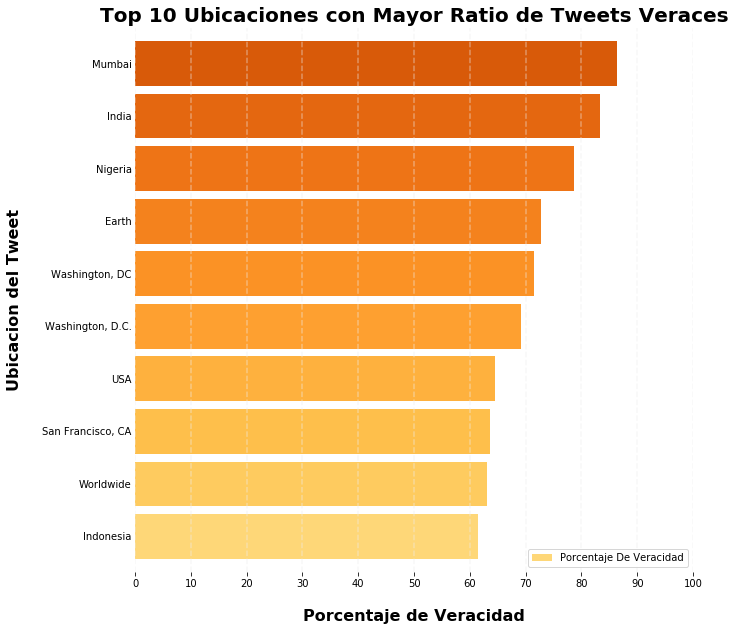
\includegraphics[width=1\textwidth]{graficos/Analisis de Locacion/top_10_locaciones_con_mayor_ratio_de_tweets_veraces.png}
    \caption{} 
    \end{figure}
    
    Se puede apreciar que los Tweets de India (Mumbai es una ciudad de India) tienen el mas alto porcentaje de veracidad. 
    
    De manera similar, se analiza las locaciones con mayor ratio de Tweets sin relación con desastres (Tweets falsos). 
    
    \begin{figure}[H]
    \centering
    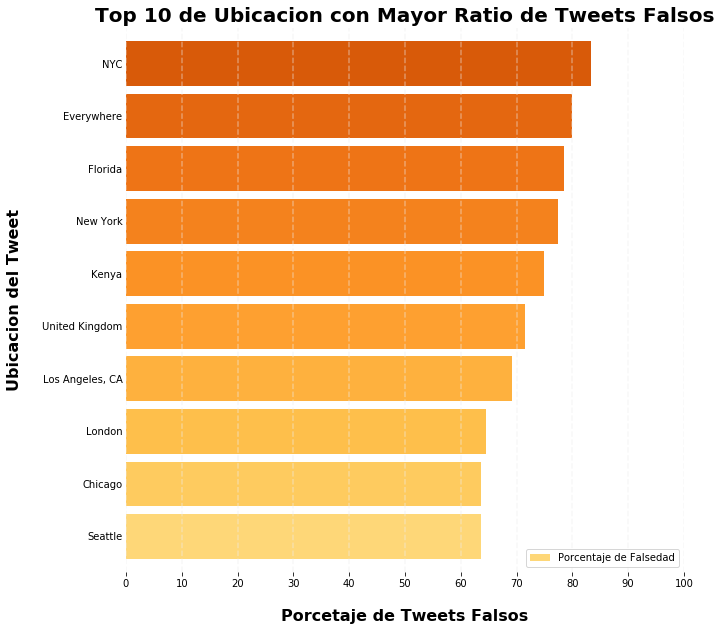
\includegraphics[width=1\textwidth]{graficos/Analisis de Locacion/top_10_locaciones_con_mayor_ratio_de_tweets_falsos.png}
    \caption{}
    \end{figure}
    
    Se puede apreciar una importante presencia de ciudades de Estados Unidos en el Top (6 de las 10 entradas). 
    
    Debido a la variedad de locaciones observadas en estos gráficos y al problema de los sinónimos previamente mencionado, se decidió agrupar los Tweets según la ciudad, para posteriormente agruparlos por país de procedencia y, de acuerdo a ello, llevar a cabo los siguientes mapas coropléticos (en inglés, choropleth). Como salvedad se debe mencionar que no fueron tomados en cuenta aquellos Tweets en los que no se especifica la ubicación, o aquellos en los que ésta es considerada como inválida.
    
    El criterio de ''válido'' utilizado es que en el campo de ''Location'' tiene que estar correctamente escrita la ciudad o país de procedencia. En base a esto y con ayuda de un csv con información de todas las ciudades del mundo se pueden agrupar los datos de todas las ciudades de cada país para obtener información del país en el que se encuentran.  
    
    En los siguientes gráficos se puede observar el porcentaje de Tweets que efectivamente hace referencia a accidentes verdaderos según el país de procedencia. En este primer gráfico se tuvieron en cuenta los países que tienen por lo menos 1 Tweet (aquellos país para los cuales no se encontraron datos aparecen en gris en el gráfico):
    
    \begin{figure}[H]
    \raggedleft
    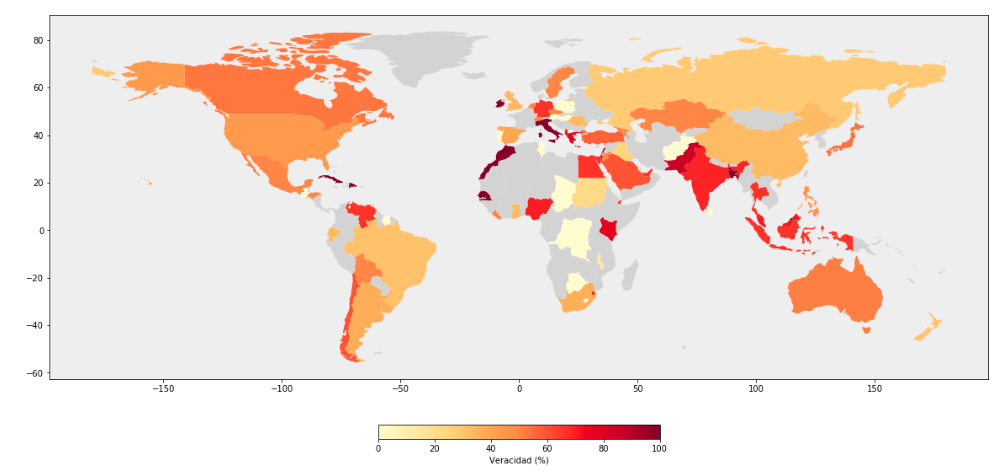
\includegraphics[width=1.1\textwidth]{graficos/Analisis de Locacion/map1.png}
    \caption{}
    \end{figure}
    
    Se observa que los países del hemisferio norte presentan una tendencia ligeramente mayor a tener un gran porcentaje de Tweets referidos tragedias reales, siendo Italia, Marruecos e Irlanda los países que predominan en éste sentido.

    Para este segundo gráfico se tienen en cuenta solo los países con por lo menos 5 Tweets. Esta decisión no es arbitraria si no que dada la cantidad de Tweets que tienen la mayoría de países y lo poco distribuidos que estos fueron tomados con respecto a todos los países del mundo (Como se explica posteriormente) se llegó a la conclusión de que esta cantidad puede representar correctamente la veracidad del país a pesar de la limitada muestra.
    
    \begin{figure}[H]
    \raggedleft
    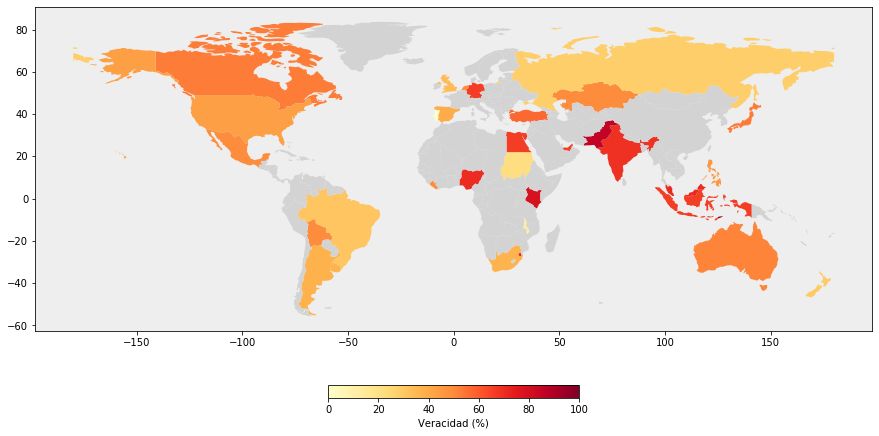
\includegraphics[width=1.1\textwidth]{graficos/Analisis de Locacion/map2.png}
    \caption{}
    \end{figure}  
    
    Como se puede observar, países como Italia, Marruecos e Irlanda, que antes figuraban con una veracidad muy alta, no fueron tenidos en cuenta en este gráfico. Puede interpretarse que los países con poca presencia en el set de datos se ven sobre-representados a ambos extremos de la curva, siendo los que más destacan con mayor y menor veracidad. El análisis de estos datos debe ser tratado con mucho cuidado pues pueden llevar a falsas conclusiones al querer generalizarlos a información de todo el país.
    
    En el siguiente gráfico se exponen los países con mayor cantidad de Tweets en escala logarítmica (en base 2):
    
    \begin{figure}[H]
    \centering
    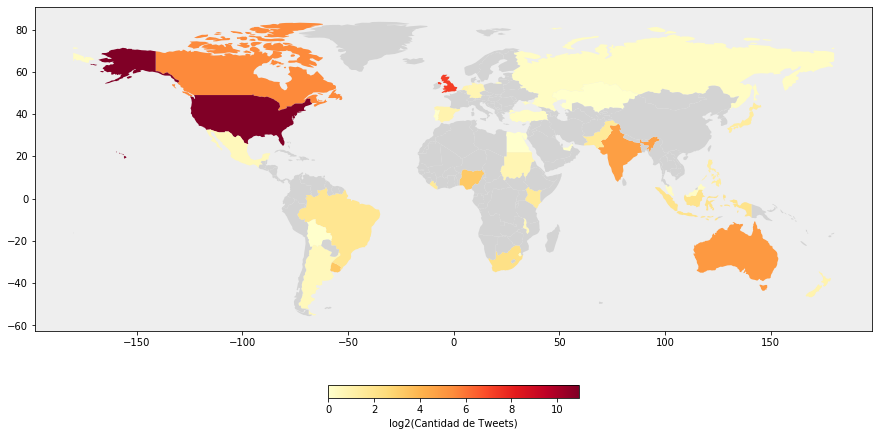
\includegraphics[width=1\textwidth]{graficos/Analisis de Locacion/map_cantidad_tweets.png}
    \caption{}
    \end{figure}
    
    El próximo gráfico muestra la misma información de manera cuantitativa:
    
    \begin{figure}[H]
    \centering
    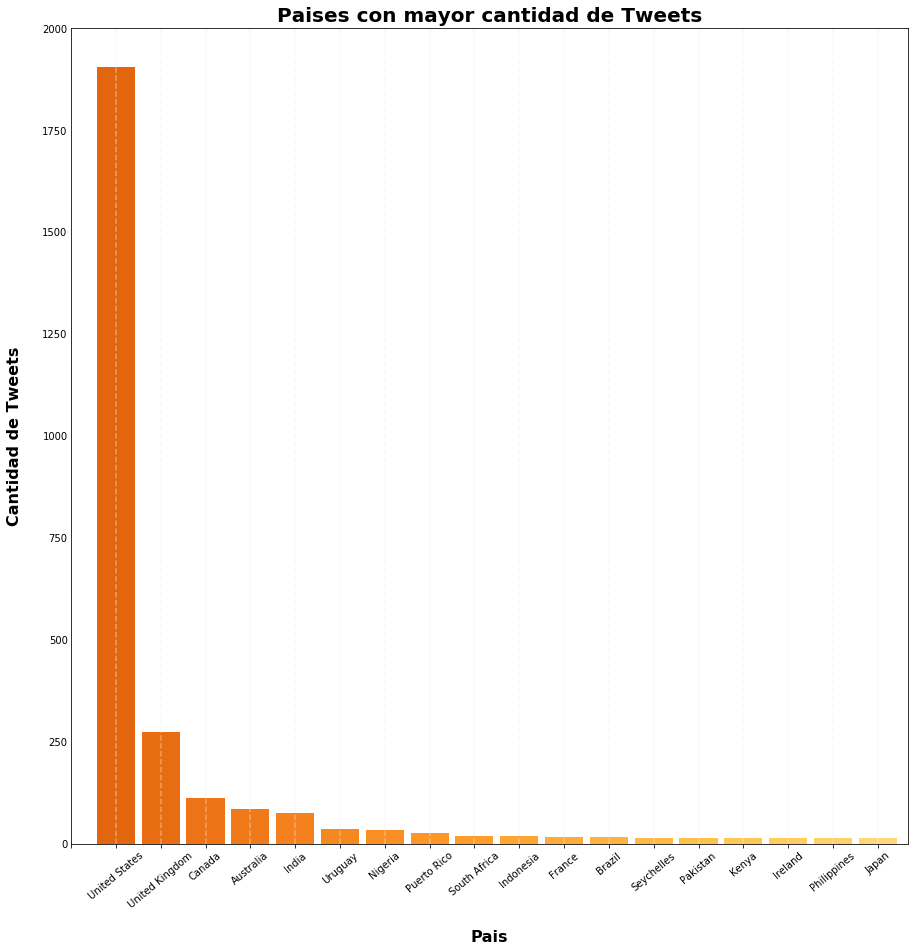
\includegraphics[width=1\textwidth]{graficos/Analisis de Locacion/paises_con_mayor_cantidad_de_tweets.png}
    \caption{}
    \end{figure}
    
    Se expone sin lugar a dudas lo mencionado anteriormente, el país con mas Tweets es con diferencia Estados Unidos. También se puede observar que prácticamente la totalidad de los Tweets provienen de países de habla inglesa. Esto puede deberse simplemente a  un sesgo al momento de recolectar los datos para el set, prefiriendo, presumiblemente, Tweets en ingles y preferentemente provenientes de Estados Unidos.
    
    A continuación, se analiza la veracidad de los Tweets por país. Para ello, se filtraron aquellos que tienen más de 10 Tweets. Esto es con el fin de que los valores obtenidos sean fieles a la realidad, y no producto de un reducido conjunto de muestras.

    \begin{figure}[H]
    \centering
    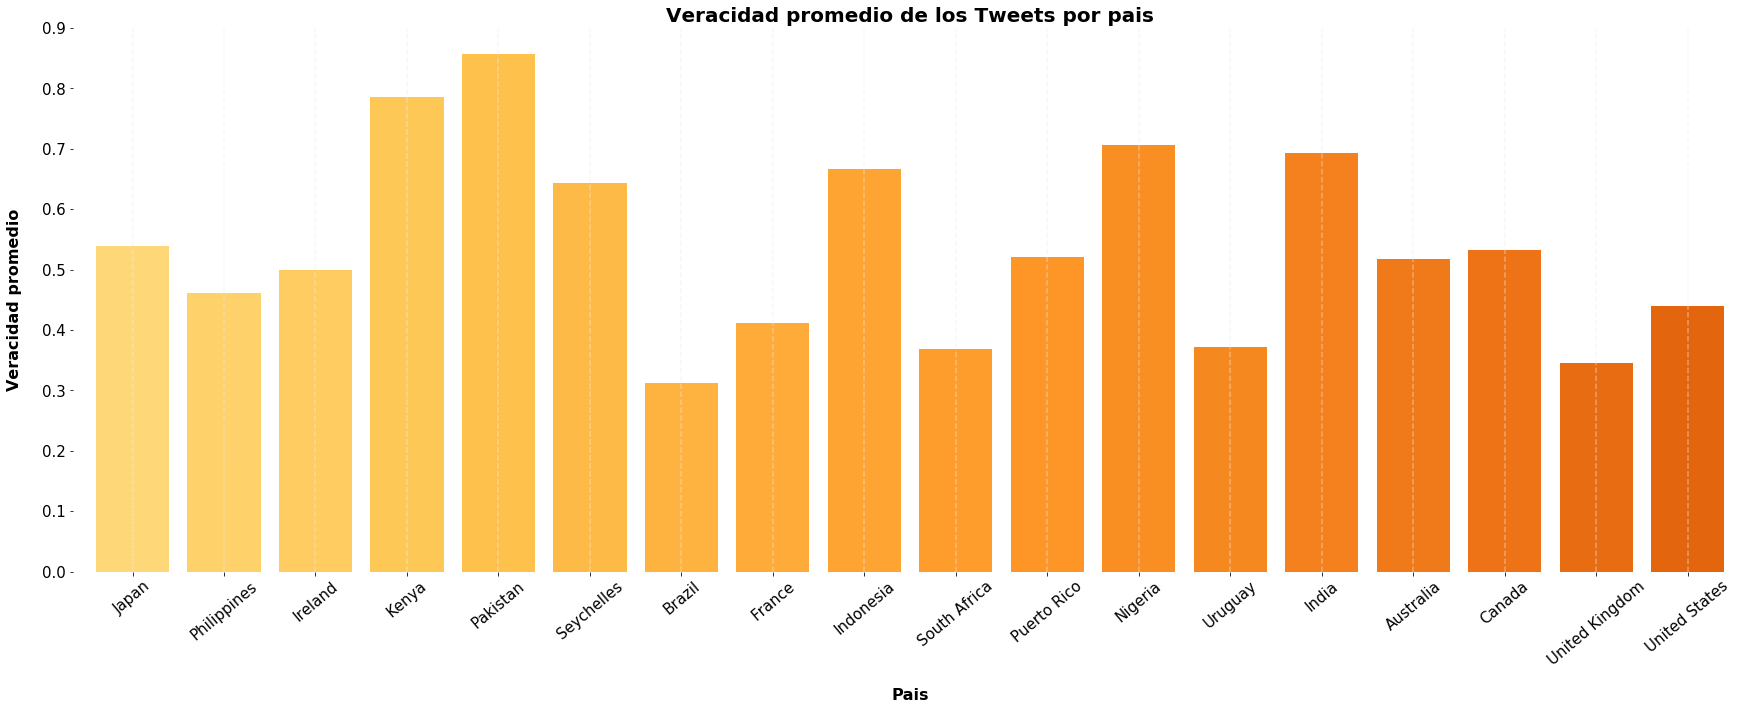
\includegraphics[width=1\textwidth]{graficos/Analisis de Locacion/veracidad_promedio_de_los_tweets_por_pais.png}
    \caption{}
    \end{figure}
    
    Como se puede observar entre los países con mayor veracidad promedio, tres de éstos pertenecen al continente africano (Nigeria, Seychelles y Kenya). Además, hay una gran representación de países asiáticos, siendo uno de ellos (Pakistan) el que presenta mayor veracidad promedio de todos los países (Con más de 10 Tweets). 
    
    De igual manera, se calcula la cantidad de Tweets por ciudad:
    
    \begin{figure}[H]
    \centering
    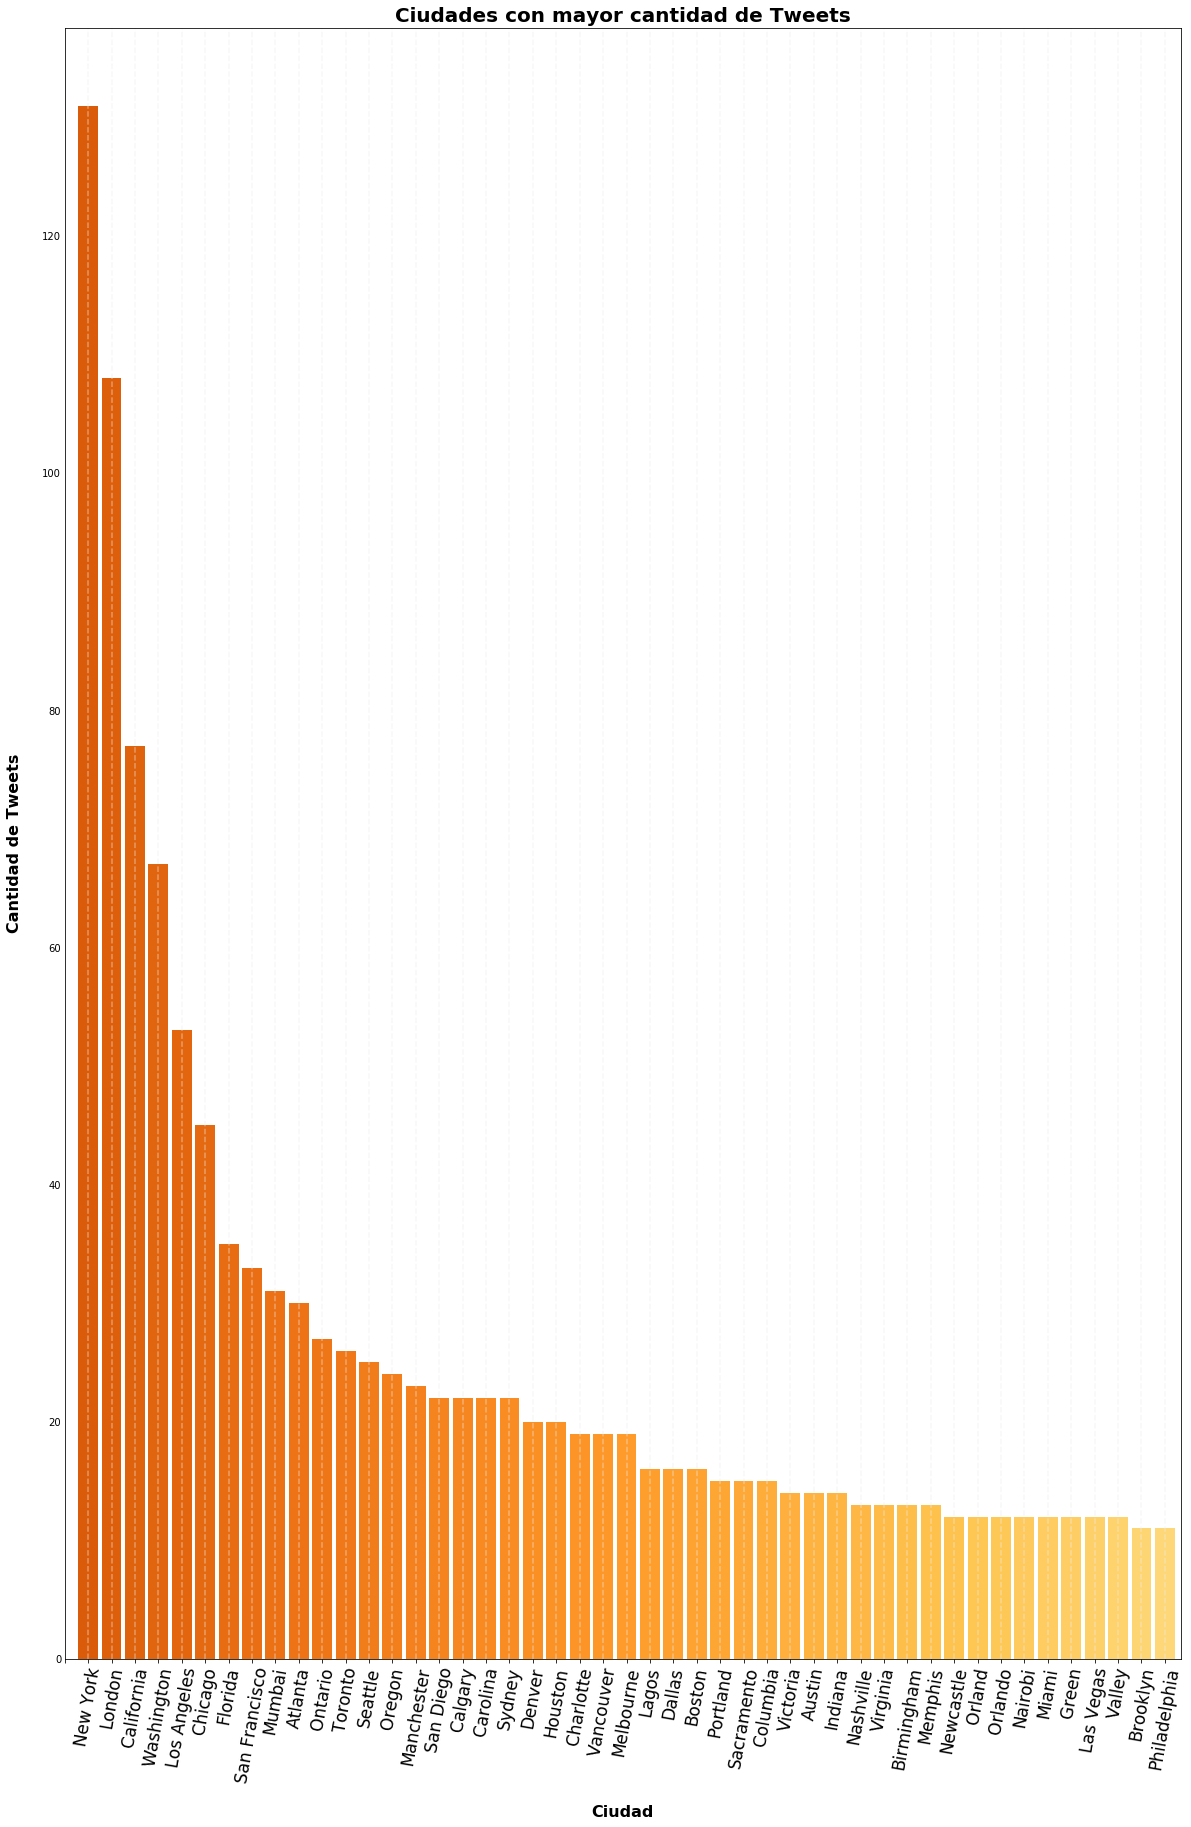
\includegraphics[width=1\textwidth]{graficos/Analisis de Locacion/ciudades_con_mayor_cantidad_de_tweets.png}
    \caption{}
    \end{figure}
    
    Este gráfico entra en concordancia una vez mas con lo mencionado anteriormente, ya que prácticamente la totalidad de estas ciudades son de habla inglesa y a su vez la mayoría de ellas se encuentran en Estados Unidos. Esto refuerza la hipótesis de cierto sesgo al momento de la recolección de datos. 
    
    Se prosigue a analizar la veracidad promedio por ciudad:
    
    \begin{figure}[H]
    \centering
    \includegraphics[width=1\textwidth]{graficos/Analisis de Locacion/veracidad_promedio_de_los_tweets_por_ciudad.png}
    \caption{}
    \end{figure}
    
    Se puede apreciar que Estados Unidos, no solo tiene ciudades con varios Tweets sino que estos también tienen una alta veracidad promedio.
    
    El siguiente gráfico expone la relación entre la veracidad y la cantidad de Tweets para cada ciudad (se tomaron las ciudades con mas de 10 Tweets por las razones explicadas anteriormente). Al mismo tiempo, el radio de los círculos es proporcional a la raíz cuadrada de la cantidad de habitantes de esa ciudad. Vale aclarar que los colores fueron elegidos arbitrariamente con el fin de ver todos los círculos a pesar de la superposición de los mismos.
    
    \begin{figure}[H]
    \centering
    \includegraphics[width=1\textwidth]{graficos/Analisis de Locacion/veracidad_vs_antidad_de_tweets_por_ciudad.png}
    \caption{}
    \end{figure}
    
    Si bien la cantidad de ciudades con una elevada cantidad de Tweets no es suficiente para sacar conclusiones con cierta certeza, se puede observar que la veracidad de las mismas tiende a un 50\%. Esto podría ser un fenómeno que ocurre en todas la ciudades como producto de aumentar el tamaño de la muestra.
    
    Otra observación importante es que las ciudades con mayor cantidad de Tweets comparten la característica de tener gran cantidad de habitantes (Círculos grandes) y las ciudades con baja cantidad de Tweets, baja cantidad de habitantes (Círculos pequeños).
    
    El siguiente gráfico es similar al anterior; pero en este caso se expone la relación entre la veracidad y la cantidad de habitantes, y en esta ocasión el radio de los círculos es proporcional a la raíz cuadrada de la cantidad de Tweets de esa ciudad. Al igual que el anterior gráfico, los colores de los círculos fueron elegidos arbitrariamente para facilitar la visualización:
    
    \begin{figure}[H]
    \centering
    \includegraphics[width=1\textwidth]{graficos/Analisis de Locacion/veracidad_vs_cantidad_de_habitantes_por_ciudad.png}
    \caption{}
    \end{figure}
    
    A diferencia del anterior gráfico, este muestra que mientras más habitantes tiene la ciudad, más tiende a tener alrededor del 50\% de veracidad. También es fácil notar que prácticamente no hay ciudades con veracidad mayor al 80\%.
    
    TITULO ACA?
    
    En los siguientes gráficos se exponen las palabras mas usadas en los países con mayor cantidad de Tweets, cada uno acompañado de una imagen mas llamativa visualmente para representar esto mismo no tan cuantitativamente, en los cuales el tamaño de la palabra representa la cantidad de apariciones que tiene dentro de los Tweets que corresponden a ese país.
    
    \begin{figure}[H]
    \centering
    \includegraphics[width=1\textwidth]{graficos/Analisis de Locacion/10_palabras_mas_usadas_usa.png}
    \caption{}
    \end{figure}
    Se puede apreciar que todas las keywords están en ingles, lo cual es esperable debido a ser el idioma nativo del país.

    \begin{figure}[H]
    \centering
    \includegraphics[width=1\textwidth]{graficos/Analisis de Locacion/bandera_usa.png}
    \caption{}
    \end{figure}
    
    \begin{figure}[H]
    \centering
    \includegraphics[width=1\textwidth]{graficos/Analisis de Locacion/10_palabras_mas_usadas_uk.png}
    \caption{}
    \end{figure}
    
    Al igual que con lo ocurrido con Estados Unidos, todas las Keywords están en ingles, lengua nativa del pais.
    
    \begin{figure}[H]
    \centering
    \includegraphics[width=1\textwidth]{graficos/Analisis de Locacion/bandera_uk.png}
    \caption{}
    \end{figure}

    \begin{figure}[H]
    \centering
    \includegraphics[width=1\textwidth]{graficos/Analisis de Locacion/10_palabras_mas_usadas_canada.png}
    \caption{}
    \end{figure}
    
    
    \begin{figure}[H]
    \centering
    \includegraphics[width=1\textwidth]{graficos/Analisis de Locacion/bandera_canada.png}
    \caption{}    
    \end{figure}
    
    \begin{figure}[H]
    \centering
    \includegraphics[width=1\textwidth]{graficos/Analisis de Locacion/10_palabras_mas_usadas_australia.png}
    \caption{}
    \end{figure}
    
    \begin{figure}[H]
    \centering
    \includegraphics[width=1\textwidth]{graficos/Analisis de Locacion/bandera_australia.png}
    \caption{}
    \end{figure}
    
    \begin{figure}[H]
    \centering
    \includegraphics[width=1\textwidth]{graficos/Analisis de Locacion/10_palabras_mas_usadas_india.png}
    \caption{}
    \end{figure}
    
    Es esperable que una de las Keywords mas usadas en India sea ''mh370''. Como ya se comento, esta esta relacionada con el vuelo 370 de Malaysia Airlines. Dentro de este vuelo se encontraban cinco pasajeros de nacionalidad Hindú. Además de haber sido uno de los países que aportaron que se sumo rápidamente a los esfuerzos internacionales de búsqueda del aeronave. Otra Keyword que puede estar relacionada con el accidente mencionado es ''Malaysia''.
    
    \begin{figure}[H]
    \centering
    \includegraphics[width=1\textwidth]{graficos/Analisis de Locacion/bandera_india.png}
    \caption{}
    \end{figure}
    
    
    Es destacable que la Keyword ''Fire'' aparece en todas los cinco países analizados. La presencia de esta Keyword se muestra principalmente en Canadá y en Australia, ambos países que suelen tener incendios forestales. 
    
    También se observa que de las Keywords de los cinco países se encuentran en ingles, lo cual no es extraño en Estados Unidos, Reino Unido, Canadá ni Australia debido a que en dichos países el ingles es la lengua nativa pero en India este no es el caso. Esto se puede deber a cierto sesgo previamente mencionado al momento de la recolección de datos. 

    \newpage
    \section{Conclusión}\label{sec:intro}
    
    
\end{document}

